% ===========================================================================
% paper.tex
%
% Master LaTeX file for the paper. Each Section lives in its own file;
% this master wraps the preamble + \input{}s. Sections not yet drafted
% appear as stub \section headers with a visible PLACEHOLDER note.
%
% To build:
%   cd paper && latexmk -pdf paper.tex
% or:
%   pdflatex paper && bibtex paper && pdflatex paper && pdflatex paper
%
% The planned paper (coauthor's Quip draft) is mirrored in paper_planned.pdf
% and as a text-searchable Markdown in paper_planned.md.
% ===========================================================================

\documentclass[11pt,letterpaper]{article}

% ---- Page layout ----------------------------------------------------------
\usepackage[margin=1in]{geometry}
\usepackage{setspace}
\onehalfspacing

% ---- Fonts and encoding ---------------------------------------------------
\usepackage[T1]{fontenc}
\usepackage[utf8]{inputenc}

% ---- Math -----------------------------------------------------------------
\usepackage{amsmath, amssymb, amsthm}

% ---- Graphics and tables --------------------------------------------------
\usepackage{graphicx}
\usepackage{xcolor}
\usepackage{booktabs}
\usepackage{array}
\usepackage{caption}
\usepackage{float}

% ---- Citations (natbib for author-year \citep / \citet) -------------------
\usepackage[round, authoryear]{natbib}

% ---- Hyperlinks (load last) -----------------------------------------------
\usepackage[colorlinks=true, linkcolor=blue, citecolor=blue,
            urlcolor=blue]{hyperref}
% Clickable DOIs. plainnat emits \doi{...} in the .bbl via \providecommand,
% so this definition takes precedence (doi.sty is not in this TeX Live).
% Verbatim-safe: % and # are set to catcode 12 (other) BEFORE the argument
% is tokenized (the doi.sty pattern), so hostile DOIs need no escaping.
% Limitation shared with all verbatim-style macros: \doi cannot appear
% inside another macro's argument — fine for .bbl entries, which call it
% at top level. Verified against 10.1000/weird%20case#frag (PR chore/
% repo-hygiene test compile). If doi.sty is ever installed and
% \usepackage{doi} added, DELETE this whole block first (the
% \newcommand will clash with the package's definition).
\makeatletter
\newcommand{\doi}{\begingroup \catcode`\%=12 \catcode`\#=12 \@doi}
\def\@doi#1{doi: \href{https://doi.org/#1}{\nolinkurl{#1}}\endgroup}
\makeatother

% ---- Paths ----------------------------------------------------------------
\graphicspath{{../results/figures/}{figures/}}

% ---- AutoFill scalars -----------------------------------------------------
% Generated by code/analysis/generate_scalars.R. Loaded here with IfFileExists
% so the paper still compiles if scalars.tex hasn't been generated yet.
\IfFileExists{../results/scalars.tex}
  {\input{../results/scalars.tex}}
  {\typeout{WARNING: ../results/scalars.tex not found. Run Rscript code/analysis/generate_scalars.R first.}}

% ---- Commands for placeholders (visible in draft) -------------------------
\newcommand{\placeholder}[1]{\textcolor{red}{\textbf{[PLACEHOLDER:} #1\textbf{]}}}

% ---- Title ----------------------------------------------------------------
\title{Transport Restructuring and Regional Development:\\
       Evidence from Argentina, 1960--1991\\[0.5em]
       \large (Working title; alternatives under discussion)}
\author{Jos\'e Belmar\thanks{Brown University.}\\[-0.2em]
        \and Diego Gentile Passaro\thanks{Brown University.}}
\date{\today}

\begin{document}

\maketitle

% NOTE (W17): Abstract drafted at provisional-draft assembly; numbers via
% scalars.tex macros. FLAGGED FOR COAUTHOR REVIEW -- wording not yet agreed.
\begin{abstract}
\noindent Between 1960 and 1991, Argentina closed roughly 10{,}000
kilometers of railway lines while its paved road network nearly
tripled (1954--1986), a restructuring driven by fiscal
consolidation rather than regional policy. We estimate how district-level outcomes responded to
the resulting changes in market access, computed from least-cost
routes integrating both modes across \nDistricts{}
districts. To address endogenous network placement, we instrument with
the technical closure rules of the 1962 Larkin Plan, a World
Bank-backed assessment of the transport network, and with
hypothetical road networks connecting major cities. Total population
shows a small,
marginally significant response (elasticity \mainPopCoefIVBoth{},
SE \mainPopSEIVBoth{});
manufacturing responds strongly: \mfgValprodCoefIVBoth{} for
production value, \mfgWageMassCoefIVBoth{} for wage mass;
agriculture shows no response. The population estimate, though not the
sectoral contrast, is sensitive to the trade-elasticity calibration.
Counterfactual decompositions attribute
similar estimates to rail and road;
roughly half of the response operates through
own-district infrastructure rather than regional connectivity.
\bigskip

\noindent \textbf{Keywords:} Regional Development, Market Access,
Transport Infrastructure, Railroads, Highways, Fiscal Consolidation,
Argentina

\noindent \textbf{JEL Codes:} R12, R42, N76, O18, H54
\end{abstract}

\begin{center}
\placeholder{Abstract drafted for coauthor review; wording not yet
agreed}
\end{center}

\clearpage

% ---- Drafted sections -----------------------------------------------------
% ===========================================================================
% Section 1: Introduction
%
% Ported from paper/paper_planned.pdf (the authoritative coauthor draft).
% Follows Shapiro's contractual-intro template (see Plan/foursteps.pdf):
%   ¶1-2 Motivation        ¶3-4 Challenges         ¶5 This paper
%   ¶6-7 Model/framework   ¶8-9 Data               ¶10-11 Methods
%   ¶12-13 Findings        ¶14-15 Contributions    ¶16-17 Roadmap
%
% PLACEHOLDERS (all authored by coauthors; preserve as-is):
%   - Paragraph on main findings (pending MA regressions)
%   - Paragraph on counterfactual findings (pending Block 2)
%   - Paragraph on mechanisms findings (pending Block 2)
%   - Numbers in square brackets (pending AutoFill): [10,000], [18,000],
%     [312]
% ===========================================================================

\section{Introduction}
\label{sec:intro}

How do large-scale transport infrastructure changes reshape regional
economies? While most research examines infrastructure expansions
designed to promote development, governments often face a different
challenge: fiscal consolidation that forces difficult choices about
which infrastructure to maintain. Argentina's experience between 1960
and 1991 provides a unique window into this question. Facing severe
fiscal pressure, the government implemented a massive transport
restructuring: closing [10{,}000] kilometers of railway lines while
expanding paved roads by [18{,}000] kilometers. This episode offers
rare evidence on how fiscal consolidation-driven infrastructure
changes—rather than development-oriented investments—affect regional
market access and economic outcomes.

This setting is valuable for two reasons. First, it speaks to a
policy-relevant question: when governments must cut infrastructure
spending, how do these cuts reshape the economic geography? The
Argentine plan, motivated by fiscal rationalization rather than
regional development goals, effectively acted as an unintended
industrial and regional policy by shifting the dominant transport
mode from rail to road. Second, it provides an opportunity to estimate
how regional outcomes respond to market access changes in a multimodal
infrastructure shock. Unlike typical infrastructure studies that
examine single-mode expansions, Argentina's bundled rail-road
restructuring allows us to study elasticities of population and
sectoral employment to market access changes that integrate both
transport modes.

Estimating the causal effects of such infrastructure changes faces
two fundamental challenges. First, infrastructure placement and
removal decisions are endogenous. Even when motivated by fiscal
consolidation, governments may close lines in already-declining
regions or expand roads where growth is expected. This makes it
difficult to separate the causal effect of market access changes
from pre-existing economic trends.

Second, when both rail and road networks change simultaneously, their
effects are difficult to disentangle. The changes are often spatially
correlated—regions losing rail access may or may not gain road
access—creating multicollinearity problems if we try to estimate
mode-specific effects in a single regression. Moreover, the
theoretical framework suggests that what matters for regional
outcomes is total market access integrating all transport modes, not
the separate contribution of each mode. This raises a methodological
question: what can and cannot be identified about mode-specific
effects in multimodal infrastructure episodes?

This paper addresses these challenges by studying Argentina's
transport restructuring through the lens of market access. We
construct a unified market access index that integrates both rail and
road networks using a standard spatial economics framework, computing
generalized transport costs and shortest-path routes on the historical
networks. Our main analysis estimates how regional outcomes—population,
sectoral employment, and economic activity—respond to changes in
total market access induced by the observed infrastructure plan. We
then use counterfactual market access measures to explore the relative
roles of rail closures versus road expansion, constructing separate
scenarios where only rail changes (roads frozen) or only roads change
(rail frozen).

Our empirical framework follows the market access approach standard
in spatial economics and trade. We model each district's economic
outcomes as functions of its market access, defined as the
population-weighted sum of inverse generalized transport costs to all
other districts. To address endogeneity, we instrument for observed
market access changes using two sources of variation. First, we
exploit the Larkin Plan's technical rules: the World Bank study that
motivated the reforms only examined railway segments below a specific
freight threshold for potential closure, creating a discontinuity in
closure probability. Second, we construct hypothetical road networks
connecting major cities via least-cost paths, which predict road
expansion but are orthogonal to local economic shocks.

We construct a novel dataset combining historical transport networks
with census data at the district level, covering [312] districts
across Argentina. We validate our identification strategy with
pre-period balance checks, pre-trend tests, spatial placebo tests,
and over-identification tests.

% [PLACEHOLDER paragraph on counterfactual findings --- fill in after
%  computing counterfactual MA. Expected: rail-driven MA changes
%  account for most effects. Language: "suggestive evidence." Block 2.
%  If we pursue sector-specific analysis, flag that extension here.]

% [PLACEHOLDER paragraph on mechanisms --- fill in after mechanism
%  regressions. Expected: districts losing stations/depots experienced
%  larger declines than MA alone predicts. Block 2.]

Our main results document a contrast between population and sectoral
activity. The elasticity of total population with respect to
$\Delta \ln \mathrm{MA}^{\mathrm{full}}$ is 0.046 (0.033) in the
combined-IV specification; individually, the urban, rural, and
total-population coefficients are not statistically distinguishable
from zero at conventional levels. In contrast, the elasticity of
manufacturing activity is sizable and significant: the log change in
the value of manufacturing production has an elasticity of 0.26
(0.12) and the log change in the manufacturing wage mass has an
elasticity of 0.33 (0.13). Agricultural activity, measured by the
number of farms and by total farmed area, does not respond
detectably. This pattern is consistent with the scale-economies
hypothesis introduced in Section~\ref{sec:history}: the transport
restructuring shifted the cost structure faced by different sectors
differently, with manufacturing benefiting more than agriculture.
Robustness to alternative trade elasticities, alternative
hypothetical-road instruments, and subsample choice is reported in
Section~\ref{sec:results_robustness}.

This paper contributes to several literatures. First, we provide
causal evidence on the regional effects of infrastructure
disinvestment driven by fiscal consolidation. The Argentine episode
involved not just the removal of rail infrastructure but a
technological shift in the dominant transport mode—from rail to
road—that effectively acted as an unintentional industrial policy,
reshaping the country's economic geography. Second, we contribute to
understanding mode-specific effects in multimodal infrastructure
episodes, proposing a counterfactual market access approach that
clarifies what can and cannot be identified. Third, our findings
speak to contemporary policy debates about modal shifts in transport,
as many countries face ongoing transitions between rail and road.
Fourth, we contribute to a longstanding debate in Argentine economic
history about whether railroad closures caused the decline of
hinterland towns or merely followed pre-existing trends.

The paper proceeds as follows. Section~\ref{sec:history} provides
historical context. Section~\ref{sec:data} describes data and market
access construction. Section~\ref{sec:identification} presents the
empirical strategy. Section~\ref{sec:results} reports main results.
Section~\ref{sec:counterfactuals} explores mode-specific patterns.
Section~\ref{sec:mechanisms} examines mechanisms and heterogeneity.
Section~\ref{sec:conclusion} concludes.


% ===========================================================================
% Section 2: Historical Context
%
% Ported from the authoritative PDF at Plan/paper.pdf (copied to
% paper/paper_planned.pdf). Four subsections cover the railway system
% before 1960, the Larkin Plan, the implementation of closures and road
% expansion, and the scale-economies motivation for sector-specific
% analysis.
%
% Per Shapiro Robot-mode (tasks W1-W4), this section "states facts";
% interpretation of the findings belongs in later sections. The
% pre-existing text is already in Robot mode and has been preserved
% with only minor cleanups (line-break artifacts from PDF extraction).
%
% PLACEHOLDERS:
%   - [1 paragraph on freight evidence] at the end of 2.4 — pending
%     access to the Santa Fe Railroad freight data. Coauthor note:
%     "Frame as suggestive, not conclusive."
%
% Citation keys used:
%   baumgartnerpalazzo1969, fajgelbaumredding2022, keeling1993, larkin1962,
%   lopez_waddell2007, pahowka2005, potash1969, rock1987, whitaker1954
% All keys resolve in references.bib (verified entries, PR #89).
% ===========================================================================

\section{Historical Context}
\label{sec:history}

\subsection{Argentina's Railway System and Fiscal Crisis}
\label{ssec:railway_history}

Argentina's railway network was one of the largest in the world.
Construction began in 1857 and expanded rapidly through a combination
of national capital, foreign investment—predominantly British and
French—and direct government participation extending lines into rural
areas that were not commercially profitable. By the early twentieth
century, the network exceeded 40{,}000 kilometers, designed primarily
to connect the agricultural hinterland of the Pampas, the Northwest,
and the Northeast to the port of Buenos Aires. This radial,
export-oriented design was both cause and consequence of the
agricultural export boom of the first globalization: from 1869 to
1914, Argentine real exports grew approximately 500 percent
\citep{fajgelbaumredding2022}. By the start of the First World War,
Argentina was the eighth richest country in the world.

Starting in the 1930s, export growth slowed considerably and profit
margins of railroad companies declined. Investment in railroad
infrastructure stalled, and the aging network experienced rising
operational costs. Railroads also began to face competition from the
automotive industry—Ford produced the first Model~T in Latin America
in Buenos Aires in 1925. In 1932, Law 11.658 created a National Trunk
Road System and a lump-sum fuel tax whose proceeds were allocated
entirely to road construction and improvement; by 1935, there were
almost 3{,}000 kilometers of paved roads. During the Second World War,
Argentina remained neutral and its young industrial sector flourished
while factories in the developed world were retooled for war
production. Railroads experienced a ``second life'' as wartime food
shortages drove up international prices for Argentine agricultural
exports, helping the country accumulate reserves of \$1.6~billion
\citep{whitaker1954}. But by 1945, industry's contribution to GDP
surpassed that of agriculture for the first time \citep{potash1969}.

Supported by unions, the military, and the new industrial
bourgeoisie, General Juan Domingo Perón reached the presidency in
1946. His economic policy rested on three pillars: strengthening the
domestic market, centralized planning with state ownership of
strategic sectors, and industrial development
\citep{whitaker1954, pahowka2005}. The showcase of this program was
the acquisition and nationalization of the private railroad companies
in 1947 for \$600~million—a purchase widely debated at the time, with
economists including Raúl Prebisch arguing that the price was
excessive given the crumbling state of the infrastructure
\citep{rock1987}. By the early 1950s, when the fortuitous advantages
of the war years had faded, Argentina's economy slipped into
depression. Perón moved to protect nascent industry, armoring the
automotive and petrochemical sectors against international
competition. The road network continued to grow at a slow, steady
pace, reaching 9{,}000 kilometers of paved roads by 1955. The railroad
network, meanwhile, remained stable at around 43{,}500 kilometers, but
with a shrinking budget it suffered from poor maintenance and aging
equipment.

In 1955, a coup removed Perón from government, and the country
endured several years of political and economic instability. In 1958,
Arturo Frondizi was elected president in an election from which Perón
was banned. Frondizi's economic plan centered on fostering
industrialization through foreign direct investment: Decree 3693 of
1959 promoted investment in the national automotive industry, and 23
new factories were approved within a year. His administration was
equally aggressive in promoting road construction. In 1958, the
lump-sum fuel tax was replaced by a 35 percent ad valorem tax
(Decreto Nacional 505/1958), and in 1960 Law 15.274 instituted a
sales tax on vehicles—in both cases, funds were permanently allocated
to road construction and improvement. As for railroads, Frondizi
initially sought to modernize the crumbling infrastructure, but the
investment required to achieve a modern network while maintaining its
current size was nearly prohibitive \citep{lopez_waddell2007}. By
1960, annual railroad losses had reached approximately \$280~million
per year, accounting for almost 80~percent of the federal government
deficit \citep{keeling1993}.

\subsection{The Larkin Plan (1960--1962)}
\label{ssec:larkin}

In this context, the Argentine government agreed with the World Bank
to commission a team of experts to evaluate the long-term economic
and strategic viability of the national transport infrastructure. The
team was led by General Thomas Larkin, an American expert in military
logistics who had been decorated for his efforts supplying combat
troops during the Second World War and had experience consulting on
railroad modernization in France, Germany, and Japan. Between 1959
and 1961, the World Bank mission scrutinized the profitability of the
existing railroad and road networks. The resulting study, published
by the Public Works Ministry in 1961 as \emph{Transportes
Argentinos: Plan de Largo Alcance} (``Argentine Transportation:
Long-Run Plan''), comprised three volumes totaling approximately
3{,}000 pages. The first volume contained an executive summary with
diagnosis, methodology, results, and recommendations organized by
transport mode and time horizon; the remaining two volumes, of
approximately 1{,}000 pages each, provided detailed
analysis.\footnote{We accessed physical copies of the plan at the
Mariano Moreno National Library in Buenos Aires. We scanned and
digitized two key objects: a map describing the operational railroad
network in 1960 (our baseline) and three tables describing the
diagnosis and recommendations for each railroad segment.}

In a world of cheap and stable oil prices, and given the poor
material and financial condition of the railroad system, the plan's
main recommendations were dramatic: closure of approximately
15{,}000 kilometers of railroad track (roughly 32~percent of the
existing network), dismissal of around 70{,}000 railroad employees
(from a total of approximately 200{,}000), disposal of the entire
fleet of steam vehicles, closure of most national railroad workshops
and factories, and aggressive improvement and construction of paved
roads—in some cases to substitute for closed railroad segments, but
also to create new connections in the network \citep{larkin1962}. The
plan proposed the construction of approximately 10{,}000 kilometers of
paved roads over ten years.

A key feature of the Larkin Plan's design is that it did not study
the entire railroad network with equal intensity. Due to budget
constraints and the vast size of the existing network, only railroad
segments that fell below specific freight density thresholds were
``studied'' in detail—meaning that the experts checked each
segment's explicit revenues and costs and analyzed whether closure
was warranted. The thresholds were 1~million gross tons per year of
cargo passing through a given segment, or 500 tons per kilometer per
year of cargo entering the network through a given segment. Only
39.6~percent of the railroad network was studied. For each studied
segment, the experts issued one of three recommendations: maintain,
close, or perform a new study. Crucially, the likelihood of the plan
recommending closure was much higher for studied segments than for
nonstudied ones—a discontinuity that we exploit for identification.

The plan's recommendations were announced by President Frondizi in
1961, but massive protests and strikes erupted in many cities. After
several months of clashes and social unrest, the government decided
to abandon the plan. In the short term, only approximately
1{,}000 kilometers of track were closed. However, despite being
abandoned after just a few months, the Larkin Plan was the only
long-term comprehensive study of the national transport
infrastructure for more than 30 years. It is therefore likely that
its recommendations influenced national transport policy for decades
ahead. As we document below, railroad closures in the 1960s and
1970s were approximately three times more likely for segments that
had been studied by the plan, probably because no new large-scale
study was ever undertaken to supersede it.

\subsection{Implementation: Rail Closures and Road Expansion,
            1960--1991}
\label{ssec:implementation}

The Larkin Plan marked a trend break in the evolution of both
transport networks (Figure~\ref{fig:networks}). For railroads, it
initiated a long-term disinvestment and dismantling process. For
roads, it started an almost two-decade period of aggressive
construction and improvement. These large-scale changes occurred in
a context of population growth (from 20 to 33 million between 1960
and 1991) and increasing GDP per capita (growing approximately
35~percent at an average annual rate of 0.95~percent).

Railroad closures proceeded in two distinct waves. The first wave,
from 1960 to 1966, closed approximately 4{,}000 kilometers of track
before political opposition brought the process to a halt. The
second wave came under the military dictatorship that seized power
in 1976: without union resistance, the military government ordered
the immediate closure of over 6{,}000 additional kilometers of track
between 1976 and 1979. After 1979, the network stabilized—no further
closures or new construction occurred between 1979 and 1986. In
total, the railroad network fell from approximately
43{,}500 kilometers in 1960 to approximately 33{,}500 kilometers by
1986, a reduction of roughly 23~percent.\footnote{We end our sample
period in 1991 because there was a census in that year and because
we wish to abstract from the potentially different effects of the
privatizations of large fractions of the railroad and road networks
during the 1990s.}

Road expansion, by contrast, was continuous throughout the period.
Fueled by the dedicated fuel and vehicle taxes established under
Frondizi, the paved road network grew from approximately
10{,}000 kilometers in 1954 to approximately 28{,}000 kilometers by
1986—an increase of roughly 180~percent. Gravel roads also expanded,
though more modestly. By 1986, the combined paved and gravel road
network had reached approximately 35{,}000 kilometers, roughly equal
to the remaining railroad network. Importantly, the spatial pattern
of road expansion did not simply mirror the pattern of railroad
closures: roads were not systematically built to replace closed rail
lines. As we show in Section~\ref{sec:data}, the correlation between
rail closures and road expansion at the district level is weak,
meaning that the two shocks affected largely different sets of
districts.

\subsection{Scale Economies and Sector-Mode Specialization:
            Motivation and Hypotheses}
\label{ssec:scale_economies}

A feature of the Argentine setting that motivates part of our
analysis is that railroads and roads may serve different economic
sectors, owing to fundamental differences in their cost structures.
Railroads exhibit strong scale economies: high fixed costs (track
maintenance, stations, rolling stock) but low variable costs per
ton-kilometer at high traffic density. Roads, by contrast, have more
constant returns to scale—per-unit costs decline less steeply with
volume. The Larkin Plan itself was designed around this logic: it
studied segments precisely because their traffic density was too low
for rail's scale economies to be realized.

Data from \citet{baumgartnerpalazzo1969}, who estimated transport
costs for Argentina using detailed operational data, are consistent
with this pattern. At high cargo density (1{,}000 tons per day),
railroad costs were 0.465 pesos per ton-kilometer compared to 1.000
for roads—rail was more than twice as cheap. At low cargo density
(100 tons per day), the relationship reversed: railroad costs rose
to 13.490 pesos per ton-kilometer while road costs were 8.266—road
was substantially cheaper (Table~\ref{tab:cost_params}). If these
cost differences translated into actual shipping patterns, they
would imply a natural sector-mode specialization: agricultural
products—bulky, heavy, shipped in large volumes—would fall in the
high-density regime where rail has a cost advantage, while
manufactured goods—lighter, more varied, shipped in smaller
batches—would fall in the low-density regime where road is cheaper.

% [PLACEHOLDER: 1 paragraph on freight evidence.
%  (1) Data from Santa Fe Railroad showing manufactured goods faced
%      higher effective freights than agricultural goods.
%  (2) As road network expanded, railroads specialized in bulk
%      products — share of bulk cargo increased over time.
%  (3) Cite slides Figures 2–5 for evidence.
%  This paragraph depends on having access to the freight data
%  figures. Frame as suggestive, not conclusive.]

Whether these cost differences generate meaningful mode-specific
effects on regional economic outcomes is ultimately an empirical
question. It is not obvious a priori that they do: if road
expansion sufficiently compensated for rail closures, or if firms
and workers adjusted quickly to the new transport configuration,
the sectoral composition of economic activity might not have
changed. We treat the existence of mode-specific effects as a
hypothesis to be tested in Sections~\ref{sec:results} and~\ref{sec:counterfactuals},
rather than as an established fact. The cost data presented here
motivate the hypothesis but do not settle it.


% ===========================================================================
% Section 3: Data
%
% Per Shapiro Robot-mode writing conventions:
%   - State facts; do not argue. Interpretation belongs in Section 5.
%   - Define every concept before using it.
%   - No forward references to undefined constructs.
%   - Plain, precise language.
%
% All numerical claims in this section trace to either:
%   - code/base/*/clean_*.R                (raw network / census totals)
%   - code/pipeline/03a_build_cost_raster.R (cost-surface parameters)
%   - code/pipeline/04_market_access.R     (MA computation)
%   - data/derived/05_panel/departments_wide_panel.parquet (panel stats)
%
% Numbers marked "FROM PANEL" are pulled directly from the estimation
% panel's manifest; those marked "FROM NETWORK" come from
% rails_by_district.parquet or roads_by_district.parquet.
%
% Panel-derived statistics (population means/totals, MA distribution,
% counterfactual component means, 1947 coverage) are AutoFill macros
% from results/scalars.tex. Network-geometry numbers (km totals, segment
% counts) remain inline: they derive from stable raw shapefiles, not
% from the estimation pipeline.
% ===========================================================================

\section{Data}
\label{sec:data}

The empirical analysis combines three data components. Section~\ref{ssec:networks}
describes the transport network geometries and their changes between
1960 and 1986. Section~\ref{ssec:census} describes the district-level
population and economic outcomes. Section~\ref{ssec:ma} describes how
we construct market access from transport cost surfaces.

\subsection{Transport networks}
\label{ssec:networks}

We combine two georeferenced networks: the railway network at its 1979
status, which we map to 1960 and 1986 via each segment's recorded closure
status, and the paved-and-gravel road network at three cross sections
(1954, 1970, 1986).

\paragraph{Railways.}
The rail network comes from the network map in Argentina's 1979
\emph{Política Ferroviaria} report \citep{argentina1981politica},
which we digitised against official IGN geographic
references.\footnote{The report's Figure~V--5 was scanned,
georeferenced, and hand-traced in GIS; the resulting file contains
\railNSegments{} line segments. District-level rail kilometres are
computed by intersecting the segments with the district polygons, which
changes the network total by \railClipLossPct{}~percent.} This is a single
1979 snapshot: the project has no rail map at a second date, and the
periods below are reconstructed from it. Each digitised
segment carries the information needed to reconstruct the network and
to build the instrument. First, a three-way closure status: whether the
segment remained active through 1986, was closed before 1976, or was
closed during the military dictatorship (1976--1983). Two cross sections follow from the field's own
definitions: the network active in 1986, and the network standing before
the dictatorship closures. A third, 1960, requires an assumption,
because the status is undated: that the segments recorded as closed
before 1976 were still open in 1960. Second, its Larkin
Plan status: whether the segment was among the \railNStudied{} segments the
1962 Larkin Plan selected for detailed study --- segments falling
below the Plan's freight-density thresholds, whose closure it then
evaluated on explicit revenue and operating-cost grounds --- or among
the \railNNotStudied{} segments the Plan did not evaluate. For studied segments, the
digitisation also records which of the Plan's three recommendations
(maintain, close, or perform a new study) was issued.
The studied/non-studied distinction is the basis of the first
instrument (Section~\ref{sec:identification}).

Total rail kilometres fall from \railKmSixty{}
in 1960 to \railKmEightySix{} in 1986, a \railPctFall{}\% reduction. Of
the \railKmLost{}~km lost, \railKmDictatorship{}~km
(\railShareDictatorship{}\%) were closed during the dictatorship and
\railKmClosedPreSeventySix{}~km
(\railShareClosedPreSeventySix{}\%) before 1976.
Figure~\ref{fig:networks}a shows the
geography of the rail network and highlights the dictatorship closures
in red. \railNDistrictsNoRail{} of the \nDistricts{} districts have no
rail in any period;
these are concentrated in Patagonia and Tierra del Fuego.

\paragraph{Roads.}
The road network comes from a digitised comparison of
Automóvil~Club~Argentino road maps for 1954, 1970, and 1986
\citep{acamaps}. Each of the 1{,}741 digitised segments is classified
by the set of map years in which it appears, which lets us
reconstruct the paved-and-gravel network at each of the three cross
sections.\footnote{Segments that appear on the 1954 and 1986 maps but
not on the 1970 map are treated as continuously present (a
cartographic omission on the middle map). Segments absent from the
1986 map are excluded from the period totals.}
The network grows from 27{,}513~km in 1954 to 79{,}820~km in 1986, a
190\% increase.
Figure~\ref{fig:networks}b shows the road network and highlights the
segments added between 1954 and 1986 in red.
Table~\ref{tab:network_changes} summarises the network totals by
period.

\begin{figure}[htbp]
\centering
% Raster (PNG) versions of the heavy vector maps are compiled into the
% paper to keep the committed paper.pdf small (vector originals stay in
% results/figures/); see .kiro/tasks.md PDF-bloat entry.
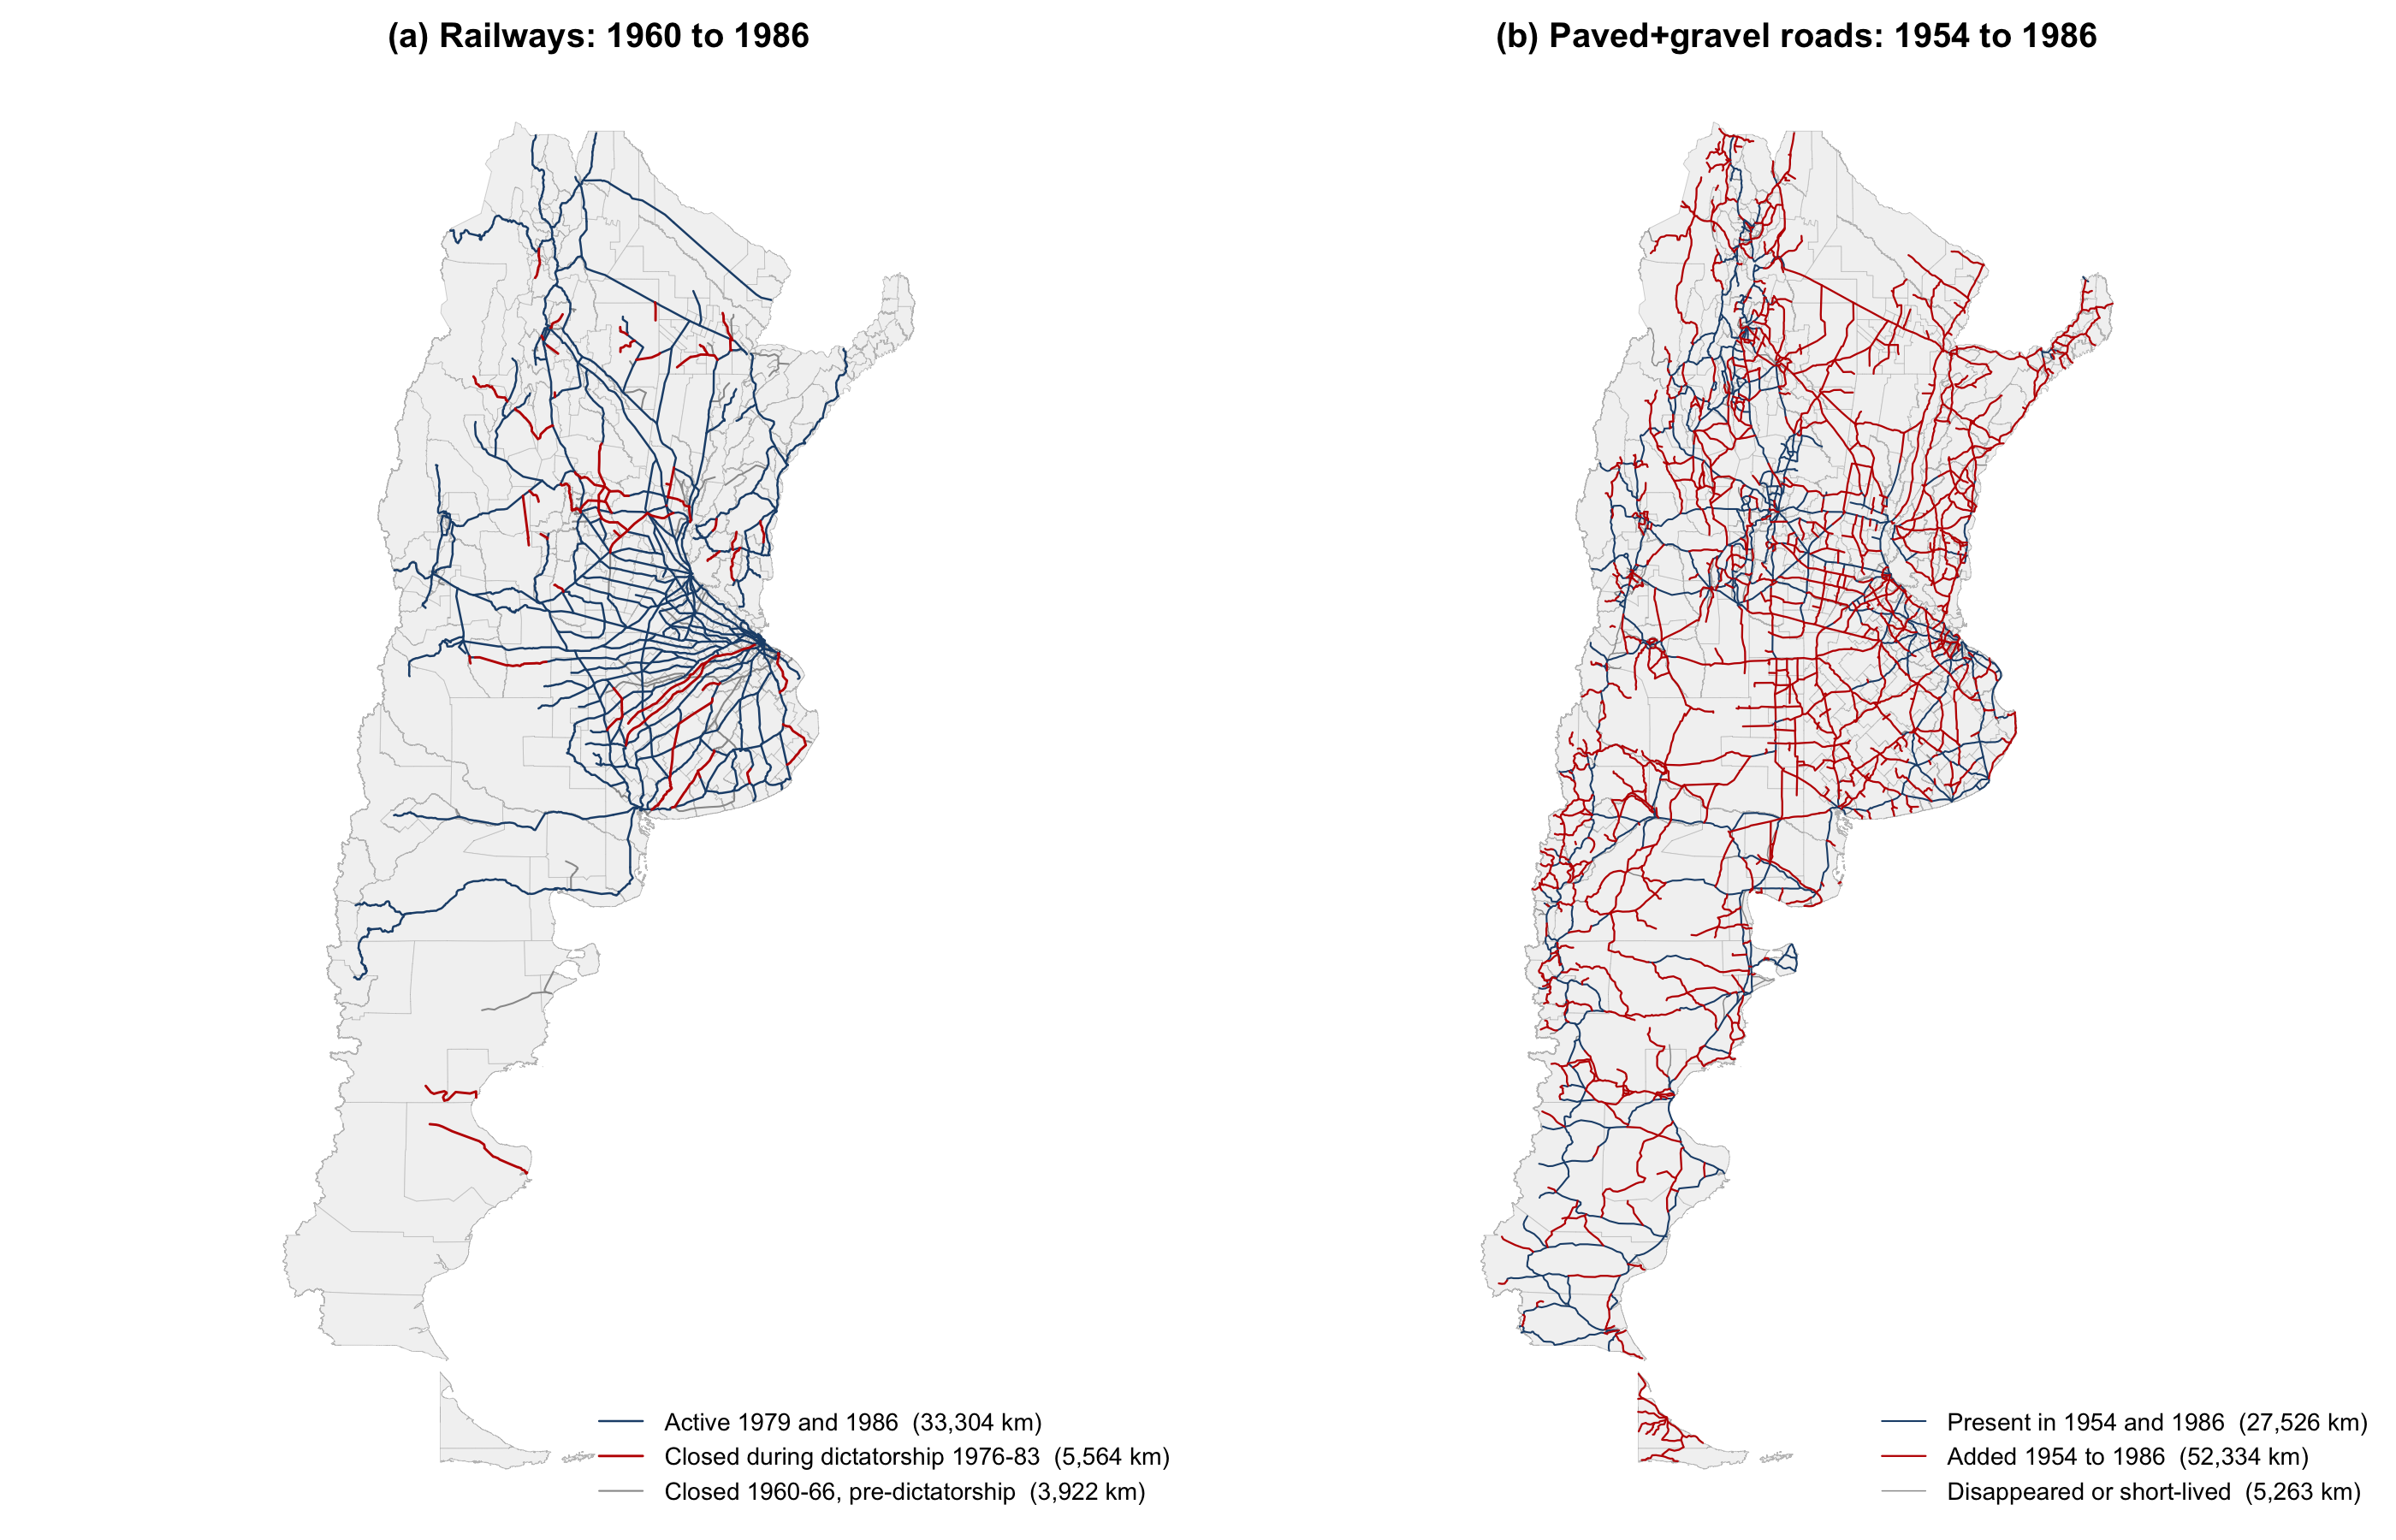
\includegraphics[width=\textwidth]{figure_1_network_changes.png}
\caption{Transport network changes, 1960--1986.}
\label{fig:networks}
\end{figure}

\begin{table}[htbp]
\centering
\caption{Transport Network Changes, 1960--1986}
\label{tab:network_changes}
\input{../results/tables/table_1_network_changes.tex}
\end{table}

Three districts, all in Patagonia, lack any segment in the road
shapefile and contribute missing values in the district-level road
variables. 11 districts lost rail without gaining roads and 141 districts
both lost rail and gained roads. The cross-district correlation between
$\Delta$(rail km) and $\Delta$(road km) is $-0.25$.

\paragraph{Hypothetical road networks.}
We also construct four hypothetical road networks that connect
Argentina's largest cities under stylised routing rules. The node set
is the 54~cities that were provincial capitals or had population of
at least 15{,}000 in 1960.\footnote{Capital Federal is not among the
nodes, although it does enter every district's market access as a
destination. The asymmetry is deliberate rather than an omission: the
market-access weights ask which destinations a district could reach,
and access to Buenos~Aires counts for all of them, whereas the
hypothetical network asks which intercity links a road programme could
have built, and Buenos~Aires is the terminus those links run to rather
than one of the cities to be connected.} The first network links every pair of
cities with a straight line (1{,}431 segments); the second is the
minimum spanning tree of those straight-line distances (53 edges).
The third replaces straight lines with least-cost paths routed over a
construction-cost surface that, following \citet{faber2014},
penalises slope, wetlands, urban land, and water crossings; the
fourth is the minimum spanning tree of those least-cost-path weights.
These networks serve as instruments for the actual road network in
Section~\ref{sec:identification}; the least-cost-path spanning tree
is the main choice, and the other three appear as robustness
alternatives.

\subsection{Census data and outcomes}
\label{ssec:census}

\paragraph{Geographic unit.}
We work at the district (\emph{departamento}) level using IPUMS
International's time-invariant district geography for Argentina
\citep{ipums2020}, which partitions the mainland into 312
districts, including Capital Federal and the two Tierra~del~Fuego
jurisdictions. The same polygons apply across the five IPUMS sample
years (1970, 1980, 1991, 2001, 2010), the 1947 and 1960 census
publications, and the agricultural and industrial censuses, so every
outcome is measured on identical boundaries throughout.

\paragraph{Population.}
Population in 1960 comes from the digitised \emph{Censo Nacional de
Población 1960} tables \citep{censo1960pop}, reconciled to the IPUMS district geography
through a crosswalk that handles pre-1960 splits and name changes. The
mean 1960 district population is \popMeanBase{} with a national total of
\popTotalBase{}~million. Population in 1991 comes from the IPUMS microdata
aggregated to the same district geography; the mean 1991 district population is
\popMeanEnd{} with a national total of \popTotalEnd{}~million. Log population change
$\Delta\log(\mathrm{pop}_{91/60})$ has mean $\chgLogPopMean{}$ and standard deviation
$\chgLogPopSD{}$. Capital Federal and the two Tierra~del~Fuego districts are
covered by both census years; Capital Federal contributes to the
market-access population weights defined in Section~\ref{ssec:ma} but
is excluded from the estimation sample as an observation
(Section~\ref{sec:results}).

\paragraph{Urban population.}
Urban population shares at the district level come from the 1960
census (classification per INDEC) and from the IPUMS 1991 microdata.
Urban population is not coded consistently in the 1970 and 2010 IPUMS
microdata for Argentina; those years are recorded as missing in the
panel and are not used for urban-outcome regressions. 1960 and 1991 give
us the post-reform window with consistent urban/rural classification.

\paragraph{Pre-reform placebo.}
We supplement the baseline with the 1947 national census
\citep{censo1947}, which covers
\placeboCoverage{} of the \nDistricts{} districts. A log population change
$\Delta\log(\mathrm{pop}_{60/47})$ for this subsample serves as a placebo
outcome: it measures population growth before any of the 1960--1986
network changes, and should be uncorrelated with the instruments if the
instruments isolate post-1960 network-induced variation.

\paragraph{Industrial and agricultural outcomes.}
Sectoral outcomes come from four additional censuses. The 1954 and
1985 industrial censuses (\emph{Censo Industrial} and \emph{Censo
Económico}; \citealt{censo1954industrial, indec1985economico}) provide
district-level establishment counts, total wages paid (the wage
mass), and production values, each measured on definitions comparable
across the two census years. Employment is recorded on incompatible
definitions in the two years (workers in 1954, total persons engaged
in 1985) and is not used. The 1960
and 1988 agricultural censuses
\citep{censo1960agro, indec1988agro} provide the number of farm
operations and total agricultural area. All monetary
variables are nominal pesos of their census year; real comparisons
across years require a deflator that we defer to robustness.

\paragraph{Geographic controls.}
District-level controls come from external sources. Area in~km$^2$ is
computed from the IPUMS polygon. Mean elevation comes from GTOPO30
\citep{usgs1996gtopo30}. Terrain ruggedness uses the Nunn--Puga TRI
raster \citep{nunn2012ruggedness} derived from GTOPO30. Wheat potential
yield comes from FAO--GAEZ~3.0 \citep{faoiiasa2012gaez}. Caloric
potential (pre-~and post-1500) comes from \citet{galorozak2016}.
Distance to Buenos Aires is the great-circle distance from the centroid
of the Gran~Buenos~Aires polygon in the IGN settlements shapefile
\citep{ignsettlements}.
All continuous controls are standardised (zero mean, unit variance) for
use in the regressions. Appendix Table~\ref{tab:descriptives} reports
descriptive statistics for every variable entering the estimation.

\subsection{Market access}
\label{ssec:ma}

\paragraph{Definition.}
Following \citet{donaldsonhornbeck2016},
we define district $i$'s market access in period $t$ for sector
$s$ under elasticity $\theta$ as:
\begin{equation}
  \mathrm{MA}_{i,t,s,\theta} = \sum_{j \neq i}
     \frac{\mathrm{pop}_{j,1960}}{(\tau_{ij,t,s})^{\theta}},
  \label{eq:ma}
\end{equation}
where $\tau_{ij,t,s}$ is the origin--destination transport cost between
the centroids of districts~$i$ and~$j$ under network configuration~$t$
and sector~$s$. Population weights are held fixed at their 1960 values
across all $t$ so that variation in~$\mathrm{MA}_{i,t,s,\theta}$ comes
entirely from variation in transport costs rather than from endogenous
population responses to the network changes. All 312 districts
contribute to the weights, including Capital Federal
(2.97~million people in 1960): access to Buenos~Aires enters every
district's market access even though Capital Federal itself is not an
observation in the estimation sample (Section~\ref{sec:results}).

\paragraph{Cost surface.}
Transport costs $\tau_{ij,t,s}$ are the least-cost-path distances on
a $2{,}399 \times 3{,}090$ raster covering mainland Argentina in the
ESRI:54034 equal-area projection (approximately 1.2~km per cell). The
per-pixel cost $c_i(t,s)$ is:
\begin{equation*}
c_i(t, s) =
\begin{cases}
\text{cost}_{\mathrm{nav}}(s)                      & \text{if pixel $i$ is navigable water,} \\
\text{cost}_{\mathrm{mininfra}}(s)                 & \text{if pixel $i$ has both rail and road,} \\
\text{cost}_{\mathrm{rail}}(s)                     & \text{if pixel $i$ has rail only,} \\
\text{cost}_{\mathrm{road}}(s)                     & \text{if pixel $i$ has road only,} \\
\text{cost}_{\mathrm{land}} \cdot \mathrm{HMI}_i   & \text{if pixel $i$ is off-network land in Argentina,} \\
\text{NA}                                          & \text{otherwise (hard barrier).} \\
\end{cases}
\end{equation*}
Network layers (rail, road, and navigation) are rasterised from the
respective shapefiles after a 1~km buffer to guarantee at least one
full raster cell per linear segment; the navigation layer comprises
the watercourse segments flagged navigable in the IGN hydrography
shapefile \citep{ignhydro}. The Strait of Magellan is buffered
by 5~km so that at least one raster cell per shore becomes navigable,
which lets Dijkstra cross the strait and keeps Tierra~del~Fuego
connected to the mainland. Off-network pixels outside Argentina are
set to NA, which acts as a hard barrier for the least-cost path
algorithm except where a navigable-water pixel overrides the country
mask (e.g.\ the Paraná river border).
Figure~\ref{fig:navigation} maps the navigation layer: the navigable
set is the inland Paraná--Paraguay--Uruguay--Río de la Plata system
plus a few Patagonian rivers, together with the Magellan crossing.
The cost surface contains no open-ocean coastal shipping, so
Atlantic ports enter the network through land or river legs only.

\paragraph{Cost parameters.}
Sector-specific cost parameters come from \citet{baumgartnerpalazzo1969}
Table~II. Three sectors $s \in \{0, 1, 2\}$ correspond to three cargo
density scenarios (medium, high, low); Table~\ref{tab:cost_params}
summarises the values.

\begin{table}[htbp]
\centering
\small
\caption{Transport Costs by Mode and Cargo Density
         (1960 pesos per ton-km)}
\label{tab:cost_params}
\begin{tabular}{lccc}
\toprule
              & Low density  & Medium density & High density \\
              & (100 t/day)  & (500 t/day)    & (1{,}000 t/day) \\
\midrule
Road          & 8.266        & 1.777          & 1.000 \\
Railroad      & 13.490       & 1.874          & 0.465 \\
Navigation    & 0.621        & 0.621          & 0.621 \\
\bottomrule
\end{tabular}

\vspace{0.5em}
{\footnotesize
\begin{minipage}{0.85\textwidth}
\emph{Notes}: Ground-transport costs from
\citet{baumgartnerpalazzo1969}. Navigation costs from
\citet{larkin1962}. Medium-density costs are used in the main
analysis (sector $s = 0$); the headline population result is
re-estimated under the high- and low-density schedules (sectors
$s = 1$ and $s = 2$) in Table~\ref{tab:density_schedules}.
\end{minipage}
}
\end{table}

In particular, rail is cheaper than road at high cargo density
($\text{cost}_\mathrm{rail}(s{=}1) = 0.465 <
\text{cost}_\mathrm{road}(s{=}1) = 1.000$) but more expensive at low
density ($\text{cost}_\mathrm{rail}(s{=}2) = 13.490 >
\text{cost}_\mathrm{road}(s{=}2) = 8.266$), which is the
scale-economies channel that motivates sector-specific analysis. At
medium density, rail and road costs are nearly identical (1.874 vs.\
1.777), so mode choice matters less for the overall market-access
index. We therefore use the medium-density scenario as the main
specification --- it is the general-purpose schedule and does not
build a mode preference into the headline treatment --- and report
the population estimates under all three schedules alongside the
main results (Table~\ref{tab:density_schedules}). The
off-network cost $\text{cost}_{\mathrm{land}}$ is
$17.9 \times \text{cost}_\mathrm{road}(s{=}2) / \overline{\mathrm{HMI}}$,
where $\overline{\mathrm{HMI}} = 0.2018$ is the national mean of the
Özak~\citeyearpar{ozak2018} Human Mobility Index. The factor~17.9 is
the ratio of motor-vehicle speed to walking-equivalent speed, calibrated
on a Buenos~Aires--Rosario comparison. This gives
$\text{cost}_{\mathrm{land}} \approx 733.2$; the per-pixel off-network
cost scales with the local HMI value and is one to two orders of
magnitude above on-network cost.

\paragraph{Least-cost path and elasticity.}
We compute $\tau_{ij,t,s}$ by running Dijkstra's algorithm over the
cost surface between the 312 district centroids, separately for each
network configuration and sector.\footnote{Paths move across an
eight-connected grid; the computation uses the \texttt{gdistance}
R~package. The replication package documents runtimes.}
$\tau_{ii,t,s}=0$ by construction and $\tau$ is symmetric.

The elasticity $\theta$ controls how sharply distant destinations are
discounted in the MA sum. It is taken from the trade literature, not
estimated in this paper. Structural
estimates span a wide range: \citet{eatonkortum2002} report a
preferred value of 8.28; \citet{simonovskawaugh2014} revise the
Eaton--Kortum approach with simulated-moments estimation and obtain
values near 4, with a credible range of roughly 4 to 8;
\citet{caliendoparro2015} estimate 8.11 for agriculture; and
\citet{donaldson2018} estimates 3.8, the only estimate from
railroad-borne trade (colonial India). We report
two values within this range, each taken from a single study:
$\theta_{\mathrm{low}} = \thetaLow{}$, the \citet{simonovskawaugh2014}
benchmark estimate (their exactly identified simulated-moments estimate
on 2004 price and trade-flow data for 123 countries, standard error
\thetaLowSE{}), and $\theta_{\mathrm{high}} = \thetaHigh{}$, the
\citet{caliendoparro2015} agricultural trade elasticity. Main results use
$\theta_{\mathrm{low}}$; $\theta_{\mathrm{high}}$
appears in the sensitivity tables, and
Section~\ref{sec:results_robustness} reports the estimates over the
full sweep $\theta \in [1, 12]$ (Table~\ref{tab:theta_sweep});
Section~\ref{sec:discussion} discusses what the sweep implies for
comparisons with the literature.
\placeholder{whether a trade-elasticity exponent is the right object
for our raw generalized cost $\tau$ is memo Decision~A, unresolved}
% THETA PROVENANCE. 8.11 traces to Caliendo-Parro's agricultural trade
% elasticity (via D&H 2016 fn. 55). The pipeline inherited theta_low =
% 4.55 with no traceable source: a provenance search (2026-07-16) found
% no occurrence in Simonovska-Waugh 2014, Caliendo-Parro 2015, D&H 2016
% fn. 55, Fajgelbaum-Redding 2022, or the old draft; Cote (2026-07-24)
% did not recall one, and 4.55 was carried as a declared midpoint.
% RESOLVED 2026-09 (Cote email, Diego approval): theta_low is now the
% Simonovska-Waugh published benchmark 4.14 (SE 0.09; their Table 5 and
% abstract; the NBER revision said 4.12 and D&H fn. 55 quote the
% overidentified 4.10). Every output regenerated; see config.R section
% 8. Memo Decision A (whether a trade-elasticity exponent belongs on a
% raw, non-normalized tau at all) is NOT resolved by citing the source
% and stays in the placeholder above.

\paragraph{Change in log MA.}
The main treatment variable is
$\Delta\log\mathrm{MA}_i \equiv \log\mathrm{MA}_{i,1986,s=0,\theta_{\mathrm{low}}}
  - \log\mathrm{MA}_{i,1960,s=0,\theta_{\mathrm{low}}}$.
Across the 312~districts,
$\Delta\log\mathrm{MA}_i$ has mean $\maMean{}$, standard deviation $\maSD{}$,
minimum $-\maMin{}$ and maximum $\maMax{}$; \maSharePos{}\% of districts see a positive
change. Figure~\ref{fig:ma_choropleth} maps $\Delta\log\mathrm{MA}_i$
across districts.

\begin{figure}[htbp]
\centering
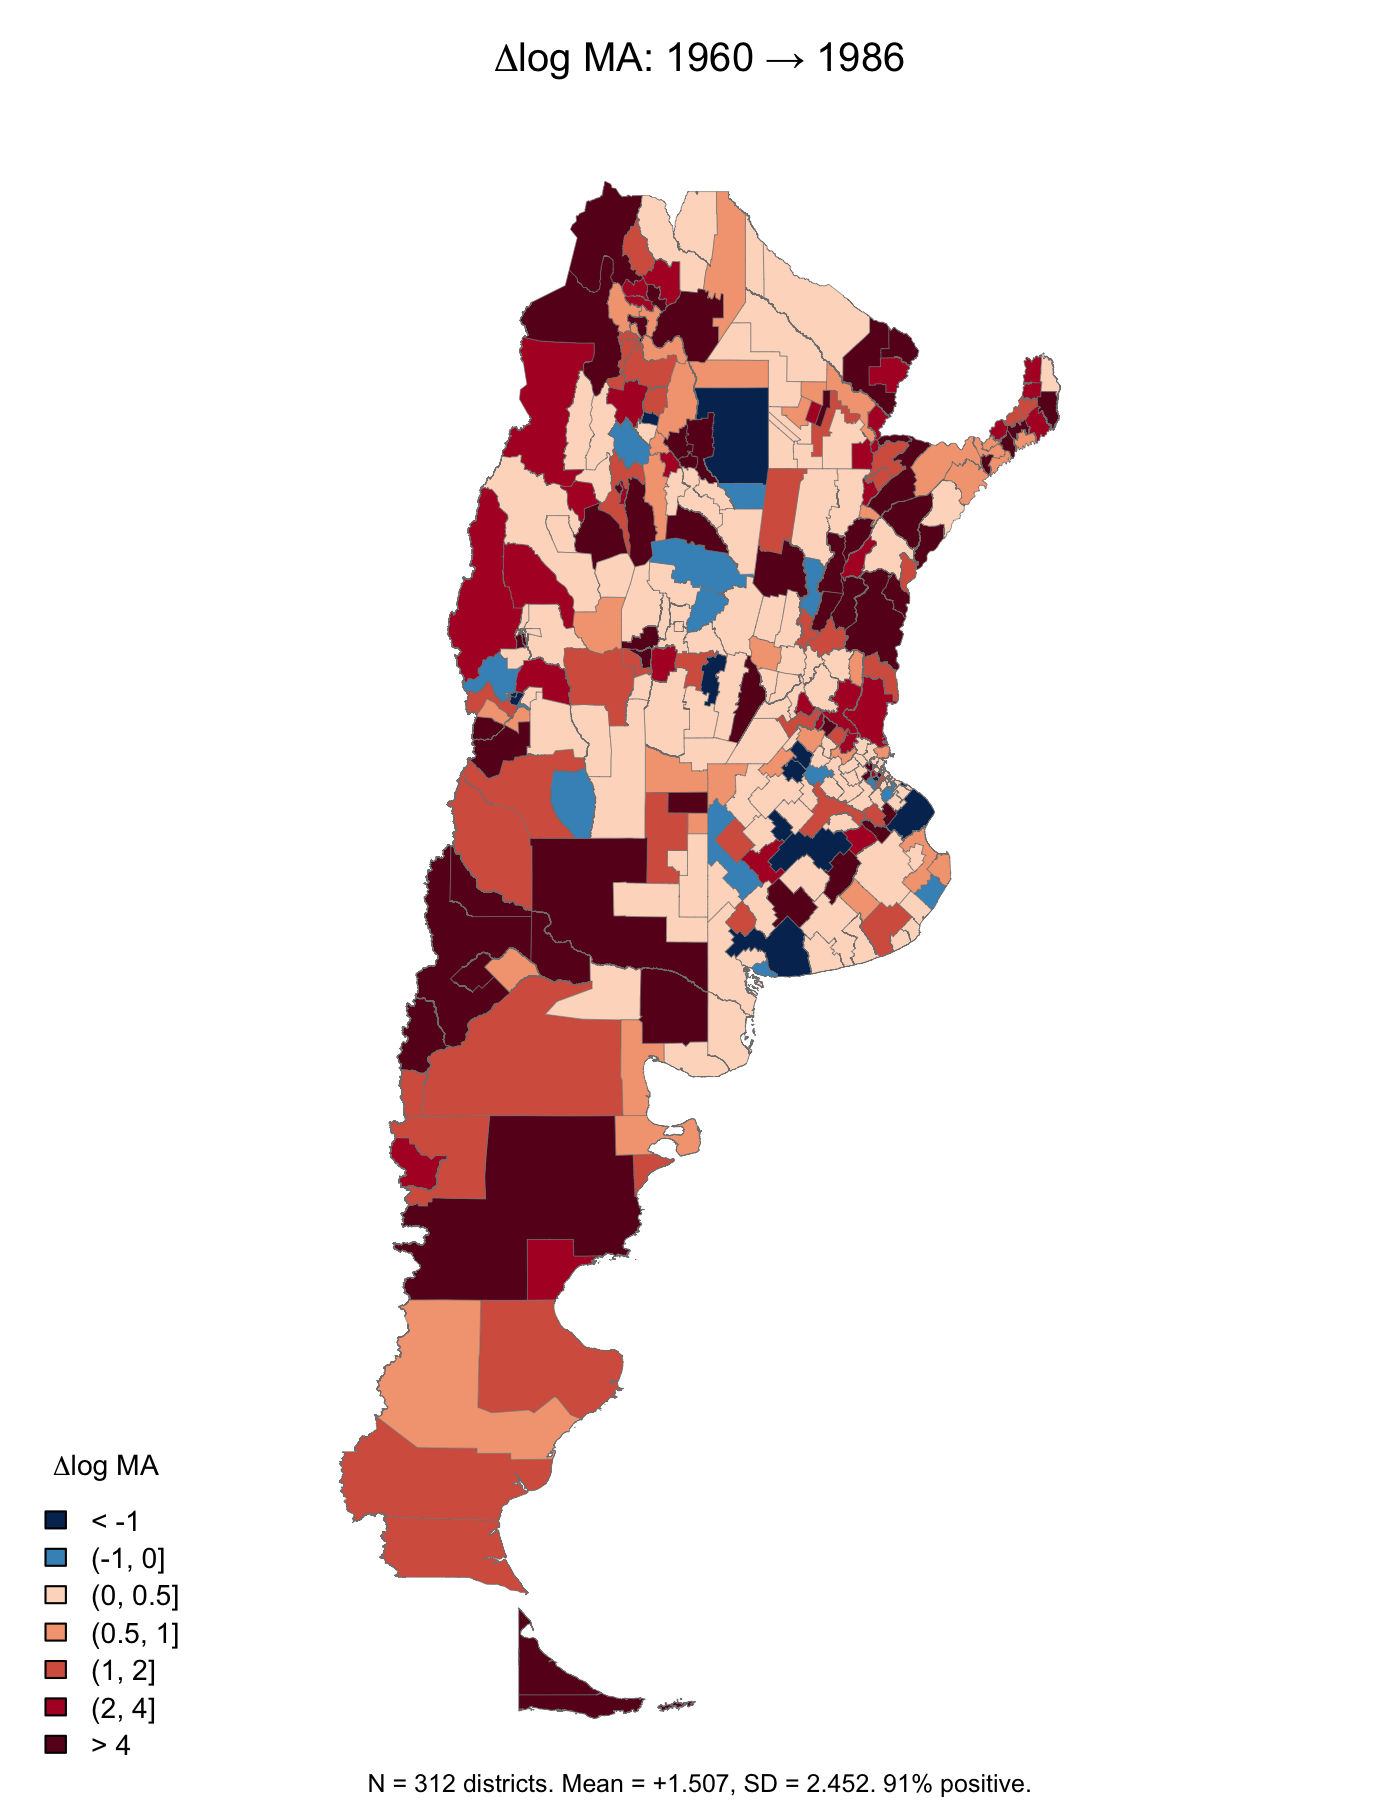
\includegraphics[width=0.85\textwidth]{figure_2_ma_change_choropleth.png}
\caption{Change in log market access, 1960--1986.}
\label{fig:ma_choropleth}
\end{figure}

\paragraph{Counterfactual decomposition.}
We additionally construct two counterfactual cost surfaces that freeze
one network mode at its baseline while letting the other change:
\begin{itemize}\setlength\itemsep{0pt}
  \item \emph{only-rail}: 1986 rails combined with 1954 roads.
  $\Delta\log\mathrm{MA}^{\text{only-rail}}_i = \log\mathrm{MA}(\text{only-rail})_i
    - \log\mathrm{MA}_{i,1960}$.
  \item \emph{only-road}: 1960 rails combined with 1986 roads.
  $\Delta\log\mathrm{MA}^{\text{only-road}}_i$ defined analogously.
\end{itemize}
At sector~0 and $\theta_{\mathrm{low}}$, $\Delta\log\mathrm{MA}^{\text{only-rail}}$
has mean $-\cfRailMean{}$ (rail contraction is a small market-access loss) and
$\Delta\log\mathrm{MA}^{\text{only-road}}$ has mean $\cfRoadMean{}$ (road
expansion is a large gain). The sum of the two isolated components
($\cfSumComponents{}$) is slightly below the total
$\Delta\log\mathrm{MA} = \maMean{}$, reflecting a positive complementarity
between the two network shocks. Figure~\ref{fig:ma_counterfactual}
compares the three maps side by side.

\begin{figure}[htbp]
\centering
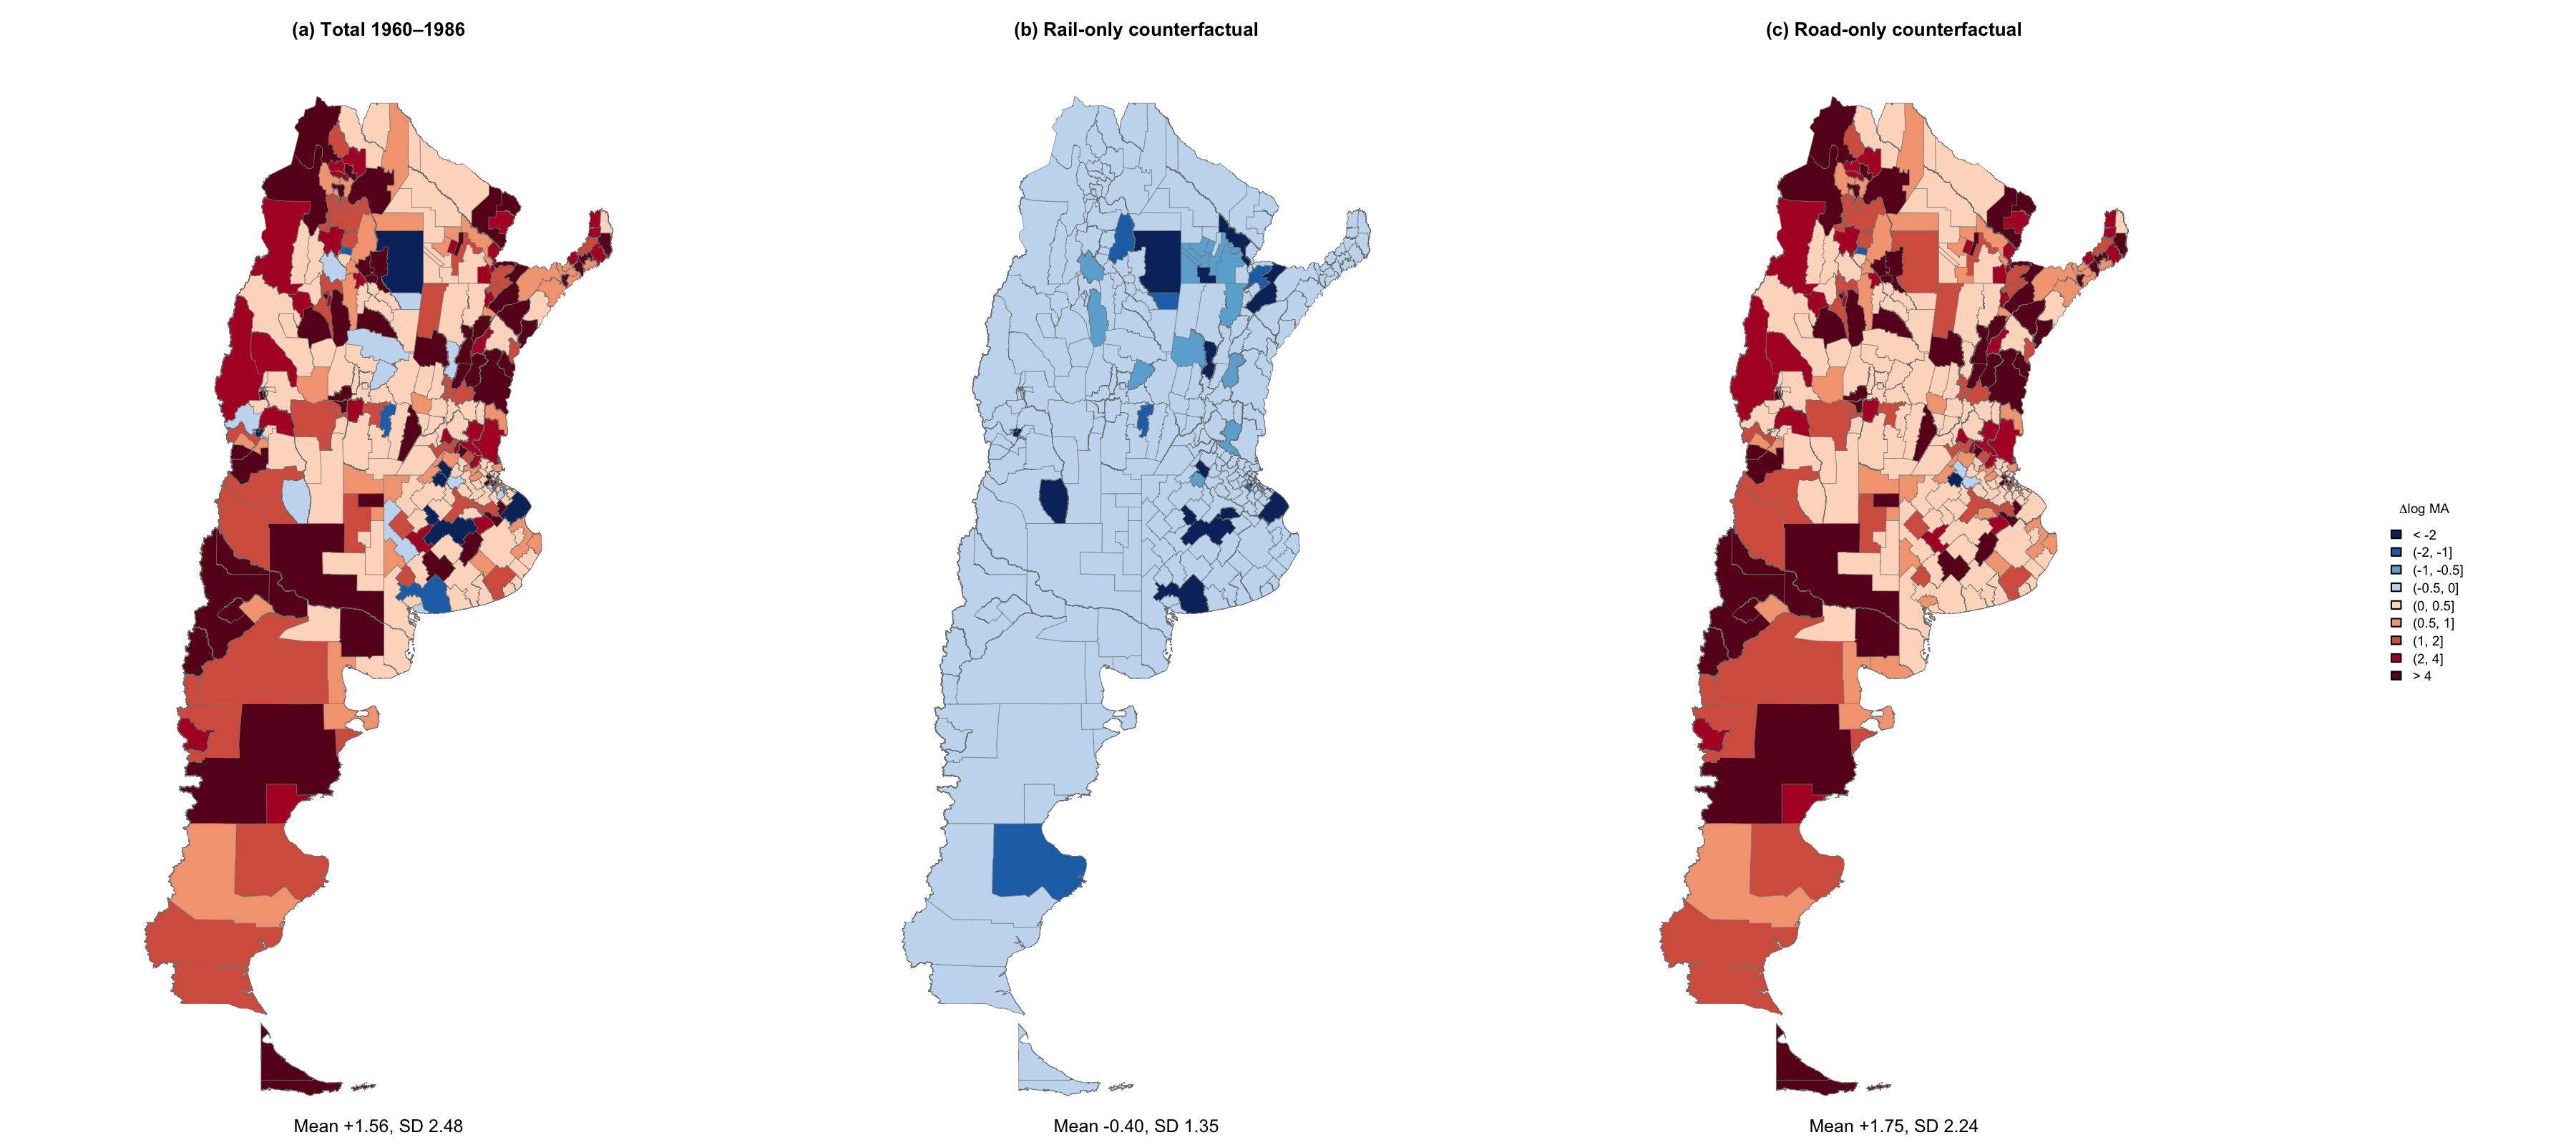
\includegraphics[width=\textwidth]{figure_c13_ma_counterfactual_trio.png}
\caption{Market access changes under three scenarios: full, only-rail
counterfactual, only-road counterfactual.}
\label{fig:ma_counterfactual}
\end{figure}

\paragraph{Limitations.}
The cost-surface construction imposes three modelling choices that the
Section~\ref{sec:identification} discussion of identification returns to.
First, mode switches are free: Dijkstra can step from a rail pixel to a
road pixel at any grid boundary, whereas in reality such switches
occur at stations or terminals and incur transshipment costs.
Section~\ref{sec:results_robustness} bounds this assumption from the
opposite extreme (one mode per trip, i.e.\ infinite transshipment
cost). Second,
the algorithm selects a single cheapest path, not a probability
distribution over routes; in equilibrium firms use multiple parallel
routes. Assigning each cell the cheapest mode deterministically also
treats modes as perfect substitutes along the path;
\citet{fuchswong2026} estimate an elasticity of modal substitution
near~1.1 between rail and truck in the contemporary United States,
far from perfect substitution.
Third, cost parameters are constant across space and time; we
do not model congestion or regional cost heterogeneity. Each of these
simplifications follows the approach in
\citet{donaldsonhornbeck2016} and is common in the market-access
literature.


% ===========================================================================
% Section 4: Empirical Strategy
%
% Ported from paper/paper_planned.pdf. The coauthor draft is partially
% written and partially scaffolded — estimating equation, first-stage
% equation, and validation-package table plans are final; several
% subsections contain author-written TODO markers flagging where
% analysis output is needed before the prose can be written.
%
% All coauthor scaffolding is preserved verbatim as LaTeX comments so
% no TODO is lost in the port. The analysis outputs that unblock the
% TODOs come from:
%   - First-stage F-stats: Phase 1/2 analysis (already in panel)
%   - Pre-period balance: Table 6 script (not yet written)
%   - Pre-trends: Table 7 script (not yet written)
%
% CITATION KEYS introduced:
%   (none beyond Section 3; equation structure reuses MA formalism)
% ===========================================================================

\section{Empirical Strategy}
\label{sec:identification}

\subsection{Estimating Equation}

Our main specification relates changes in district-level outcomes to
changes in market access:
\begin{equation}
\Delta Y_i = \beta \cdot \Delta \ln \mathrm{MA}^{\mathrm{full}}_i
             + X'_i \gamma + \varepsilon_i,
\label{eq:main}
\end{equation}
where $\Delta Y_i$ is the change in outcome, $\Delta \ln
\mathrm{MA}^{\mathrm{full}}_i$ is the change in log market access, and
$X_i$ includes baseline log market access, baseline log population, and
geographic characteristics. The parameter $\beta$ is the elasticity of
regional outcomes with respect to market access.

\subsection{Endogeneity Concerns}

The regressor $\Delta \ln \mathrm{MA}^{\mathrm{full}}_i$ is not
exogenous. The infrastructure changes that generate it --- rail
closures and road construction between 1960 and 1986 --- were policy
choices, not random assignments, and those choices plausibly responded
to the same district conditions that drive the outcomes.

The direction of the resulting bias is ambiguous because
infrastructure was allocated under two opposing logics. Under an
efficiency logic, investment follows expected growth and divestment
follows expected decline: roads are built, and rail retained, where
outcomes were already rising, while rail is closed where outcomes were
already falling. This aligns market-access gains with positive outcome
shocks and losses with negative shocks --- a positive correlation
between $\Delta \ln \mathrm{MA}^{\mathrm{full}}_i$ and $\varepsilon_i$
that biases the ordinary-least-squares estimate of $\beta$ upward.
Under a compensatory logic, investment instead targets lagging
districts --- for example, roads extended to areas that were declining
--- aligning market-access gains with negative outcome shocks and
biasing $\beta$ downward. Because both logics plausibly operated over
1960--1986, the sign of the net bias is ambiguous. We address the
endogeneity with two instruments that move market access through
variation plausibly orthogonal to district-level outcome shocks,
described next.

\subsection{Instrumental Variables}

We instrument $\Delta \ln \mathrm{MA}^{\mathrm{full}}_i$ with two
changes in market access, each computed on a counterfactual network:
one that isolates rule-based rail closure, and one that isolates
geography-driven road placement.

\subsubsection{Instrument 1: The Larkin Plan Classification}
\label{sssec:iv_larkin}

The first instrument exploits the Larkin Plan (1960--1962), the
government technical study of the rail network described in
Section~\ref{ssec:larkin}. The Plan evaluated segments against an
engineering and freight-traffic standard and designated a subset for
study toward closure; we label these segments \emph{studied} and the
remainder \emph{non-studied}, mapped in
Figure~\ref{fig:larkin_studied}.\footnote{In our cleaned data, studied
segments account for 48.8~percent of network kilometers, compared
with the 39.6~percent the report cites
(Section~\ref{ssec:larkin}). The two figures are consistent with a
definitional difference. The plan's tables assign every studied
segment one of three recommendations
(Section~\ref{ssec:larkin}), and the segments recommended for
\emph{a new study} appear not to be counted as studied in the
report's own accounting. In the raw digitized tables, where the
studied share is 49.0~percent, the new-study segments account for
5{,}197~km; excluding them, the studied share is 38.4~percent of
the approximately 43{,}500-kilometer 1960 network of
Section~\ref{ssec:implementation}. Our instrument retains these
segments: they fell below the freight-density thresholds and were
scrutinized by the plan, which is the classification the instrument
exploits.} The classification predates and is defined
independently of the regional-development outcomes we study. We
construct $\Delta \ln \mathrm{MA}^{\mathrm{LP}}_i$ as the change in log
market access between 1960 and 1986 on a counterfactual network in
which the rail segments removed are exactly those the Larkin Plan
studied, and we use it as an instrument for the realized change
$\Delta \ln \mathrm{MA}^{\mathrm{full}}_i$.

The Larkin classification predicts realized closure: studied segments
were substantially more likely to be closed than non-studied segments
(Section~\ref{ssec:larkin}), so the classification shifts the realized
change $\Delta \ln \mathrm{MA}^{\mathrm{full}}_i$, which is the
relevance condition the instrument must satisfy. The exclusion
restriction requires that the classification be uncorrelated with
district outcome shocks over 1960--1986, conditional on the controls in
equation~(\ref{eq:main}). The assumption is plausible because the Plan
applied a national, traffic-based engineering rule fixed at the start
of the period rather than a forecast of regional growth. It is not
guaranteed: if the traffic rule selected segments in districts already
on a distinct trajectory, studied status would correlate with
pre-existing trends. Sections~\ref{sec:pre_balance}
and~\ref{sec:pre_trends} probe this directly.

\subsubsection{Instrument 2: Hypothetical Road Networks}
\label{sssec:iv_hypo}

The second instrument is a hypothetical road network that connects
Argentina's major cities along the cheapest available routes,
independent of where roads were actually built. The node set is the
cities with at least 15{,}000 inhabitants in 1960 together with all
provincial capitals. We connect these nodes in two ways. Edge cost is
measured either as Euclidean distance or as the least-cost path across
a terrain-based construction-cost surface, on which steeper and more
rugged terrain is more expensive to traverse. From each cost notion we
build a minimum spanning tree --- the lowest-total-cost set of edges
that connects all cities without cycles --- which yields a parsimonious
network that does not depend on which individual city pairs happen to
be linked. This produces four variants: the full bilateral least-cost
network (LCP) and its spanning tree (LCP-MST), and the full Euclidean
network (EUC) and its spanning tree (EUC-MST); Figure~\ref{fig:hypo_networks}
maps the variants. The main specification
uses LCP-MST. We construct $\Delta \ln \mathrm{MA}^{\mathrm{hypo}}_i$
as the change in log market access induced by adding this hypothetical
network.

The hypothetical network depends only on city locations and terrain,
both fixed before the reform and unrelated to district outcome shocks
over 1960--1986. It is relevant to the extent that actual road
construction followed the same low-cost corridors connecting the same
cities; this is an empirical relevance condition, evaluated by the
first-stage fit rather than assumed. It is plausibly excludable because
the least-cost routing reflects engineering geography fixed before the
reform and does not respond to the local economic changes we study. As
with the Larkin instrument, the exclusion restriction is assessed in
the validation package (Sections~\ref{sec:pre_balance}
and~\ref{sec:pre_trends}).

\subsubsection{First Stage}
\label{sssec:first_stage}

The first stage regression is:
\begin{equation}
\Delta \ln \mathrm{MA}^{\mathrm{full}}_i
  = \alpha_1 \cdot \Delta \ln \mathrm{MA}^{\mathrm{LP}}_i
  + \alpha_2 \cdot \Delta \ln \mathrm{MA}^{\mathrm{hypo}}_i
  + X'_i \delta + u_i.
\label{eq:first_stage}
\end{equation}

\subsection{Validation Package}

Both instruments are formula instruments in the sense of
\citet{borusyakhull2023}: each is a market-access index computed from
a counterfactual network, so each combines its source of
identifying variation (the Larkin study designations; the
least-cost-routing geography) with every district's non-random
exposure to that variation through the population weights, district
locations, and the remainder of the network.
\citet{borusyakhull2023} show that instruments of this form can be
correlated with outcome shocks even when the underlying variation is
as good as random, because centrally located districts receive
systematically different instrument values than peripheral ones. The
validation exercises below address this concern directly: the balance
table asks whether the instruments correlate with predetermined
characteristics, the placebo asks whether they predict pre-period
growth, and the main specification conditions on baseline log market
access, baseline log population, and the geographic controls. These
checks partially address, but do not eliminate, the exposure concern.

Sections~\ref{sec:pre_balance} and~\ref{sec:pre_trends} present two
validation exercises that probe the exclusion restriction underlying
the two instruments. Section~\ref{sec:first_stage_tab} reports the
first stage.

A specification with two instruments and one endogenous regressor
imposes one testable restriction: both instruments must identify the
same parameter. \citet{sargan1958} gives the classical test of that
restriction. Standard errors throughout this paper are
heteroskedasticity-robust, so we also compute the
identification-robust counterpart, obtained by minimizing the
\citet{andersonrubin1949} statistic over the parameter and referring
the minimum to a chi-squared distribution with one degree of freedom.
The same statistic delivers Anderson--Rubin confidence sets, which
have correct coverage whatever the strength of the instruments; we
report them where instrument strength is in question.
\citet{andrewsstocksun2019} review both procedures. Rejection of the
restriction does not identify which instrument is at fault. It says
that the two-instrument estimate cannot be read as an estimate of a
common parameter, and that the two instruments should be reported
separately instead. Section~\ref{sec:other_outcomes} is organized
around this test, and Table~\ref{tab:other_outcomes_iv} reports it
for the four outcomes considered there.
% NOTE for Cote/Diego: Table 11 is currently the only table carrying an
% overidentification row. Adding the same row to Tables 9 and 10 is a
% two-line change (sargan_p() from code/analysis/_iv_helpers.R plus an
% add_rows entry). Deliberately not done here: it changes the headline
% tables, so it is a decision for the two of us, not a drafting call.
% Raised as an asymmetry in the PR #141 review.

\subsubsection{Pre-Period Balance}
\label{sec:pre_balance}

Table~\ref{tab:pre_balance} reports regressions of each baseline
district characteristic on the two instruments, partialling out
baseline log market access, baseline log population, and the six
geographic controls of the main specification; a characteristic that
is itself one of these controls is excluded from its own control
set. Each row is a
separate regression of the row-label characteristic; columns report
the instrument coefficients under three specifications: the Larkin
Plan instrument alone (column~1), the hypothetical-road instrument
alone (column~2), and both instruments jointly (column~3). Standard
errors are heteroskedasticity-robust.

The Larkin Plan instrument is uncorrelated with baseline log
population (column~1 coefficient $\balLPPopCoef{}$, $p\balLPPopP{}$).
It shows residual
correlations with baseline urban share ($\balLPUrbshrCoef{}$,
$p\balLPUrbshrP{}$), wheat
suitability ($\balLPWheatCoef{}$, $p\balLPWheatP{}$), pre-1500 caloric potential
($\balLPPreCalCoef{}$, $p\balLPPreCalP{}$), post-1500 caloric potential ($\balLPPostCalCoef{}$,
$p\balLPPostCalP{}$), distance to Buenos Aires ($\balLPDistBACoef{}$, $p\balLPDistBAP{}$), and log
district area ($\balLPAreaCoef{}$, $p\balLPAreaP{}$). These correlations are small in
magnitude but statistically detectable. Wheat suitability, the two
caloric potentials, and distance to Buenos Aires are controls in the
main specification, so their residual
correlations shift from exclusion-restriction threats to a
conditional-independence requirement: the Larkin Plan instrument must
be uncorrelated with the outcome \emph{conditional on} these
geographic controls.

The hypothetical-road instrument shows imbalance at the five-percent
level for \balHypoNImbalanced{} of the nine baseline characteristics
(baseline log population and log district area); the remaining
column~2 coefficients show no correlation at conventional levels.
Baseline log population is a control in the main specification. The
joint specification in
column~3 yields similar results to the single-instrument columns.

\input{../results/tables/table_6_pre_balance.tex}

\subsubsection{Pre-Trends}
\label{sec:pre_trends}

Table~\ref{tab:pre_trends} reports a placebo test. The dependent
variable is the log change in district population between 1947 and
1960 --- a change that predates the 1960--1986 infrastructure
restructuring. The regressor is $\Delta \ln
\mathrm{MA}^{\mathrm{full}}_i$ computed over 1960--1986. If the
infrastructure changes in 1960--1986 are driven by instruments
orthogonal to pre-period district-level dynamics, the coefficient on
post-reform $\Delta \ln \mathrm{MA}^{\mathrm{full}}_i$ in this
placebo regression should be near zero.

The sample is \placeboNIVBoth{} districts --- the subset for which the 1947 census
provides comparable population counts under the time-invariant
district boundaries, as discussed in Section~\ref{sec:data}. Columns~(1) to~(4)
match the structure of Tables~\ref{tab:population_iv}
and~\ref{tab:sectoral_iv}: OLS, IV-LP, IV-Hypo, IV-Both.

The controls in this table differ from those in
Tables~\ref{tab:pre_balance}, \ref{tab:first_stage}
and~\ref{tab:population_iv} in one term: the population baseline is
the 1947 level, not the 1960 level. The reason is that the outcome
here is $\ln \mathrm{pop}_{1960} - \ln \mathrm{pop}_{1947}$, so the
1960 level is the terminal value of the window under test, and
conditioning on it would mean conditioning on a component of the
outcome. The 1947 level is the initial value, a convergence control.
The baseline market-access control is retained.
Table~\ref{tab:placebo_ladder} reports the estimate under four
baseline control sets, including the set that drops the
market-access control; the estimate is sensitive to that choice, and
Section~\ref{sec:limitations} returns to it.

The OLS coefficient is \placeboOLSCoef{} (\placeboOLSSE{}), with
$p=\placeboOLSP{}$. The IV-LP estimate is \placeboIVLPCoef{} (\placeboIVLPSE{}), the IV-Hypo estimate is
\placeboIVHCoef{} (\placeboIVHSE{}), and the combined IV estimate is \placeboCoefIVBoth{} (\placeboSEIVBoth{}),
with $p=\placeboIVBP{}$. The first-stage $F$ for the
IV-Hypo column on this sample of \placeboNIVBoth{} districts is \placeboFHypo{}, below
conventional weak-instrument thresholds; the IV-Hypo column is
therefore not interpretable in this specification. The first-stage
$F$ for IV-LP is \placeboFLP{} and for IV-Both is \placeboFBoth{}.

The combined-IV point estimate for the placebo outcome is positive
and rejects a zero coefficient at the ten-percent level, though not
at five percent; the OLS estimate has the same sign and does not
reject. This is not a clean null. Two readings are
consistent with the evidence. First, there may be a genuine
pre-existing trend correlated with the eventual infrastructure
changes of 1960--1986: districts that were growing fastest in
1947--1960 may have been more likely to gain (or lose) market access
in the later period. Second, the placebo outcome is defined on a
subsample ($N=\placeboNIVBoth{}$) that is non-random with respect to the full
estimation sample ($N=\mainPopNIVBoth{}$), and the correlations documented in
Section~\ref{sec:pre_balance} for the Larkin Plan instrument may
interact with that subsample selection.

Section~\ref{sec:results_robustness} reports the main-spec population
regression refit on the same \placeboNIVBoth{}-district subsample. On that
subsample, the IV-Both coefficient on $\Delta \ln
\mathrm{MA}^{\mathrm{full}}_i$ is \subIVBCoef{} (\subIVBSE{}), with $p=\subIVBP{}$. This
coefficient is similar in magnitude to the placebo coefficient of
\placeboCoefIVBoth{} reported above. The two readings offered in the preceding
paragraph are therefore not distinguishable by this test: the pre-
reform pattern on the \placeboNIVBoth{} subset is of the same order as the
post-reform main-spec coefficient on the same subset. We retain the
main specification on the full sample as the headline estimate and
report the placebo-subsample result in the robustness panel.

\input{../results/tables/table_7_pre_trends.tex}

\subsubsection{First-Stage Results}
\label{sec:first_stage_tab}

Table~\ref{tab:first_stage} reports the first-stage regressions.
Results are described in Section~\ref{sec:first_stage}.

\input{../results/tables/table_8_first_stage.tex}

\subsection{Additional Robustness Approaches}

We assess robustness by varying the distance decay parameter
($\theta$), the set of controls, the sample (excluding major cities,
border regions), and the time period (1960--1970, 1970--1991).
Results are reported in Table~\ref{tab:robustness}.


% ===========================================================================
% Section 5: Main Results
%
% Robot-mode (Shapiro Step 3): state facts, do not argue; define concepts
% before use; no forward references to undefined constructs; plain precise
% language.
%
% Subsections drafted here (anchored by Tables 8, 9, 10):
%   5.1 First Stage
%   5.2 Population Effects
%   5.3 Sectoral Activity (renamed from "Employment and Sectoral Effects"
%       per PR #49 -- the paper-skeleton employment outcomes could not
%       be implemented; the industrial and agricultural census activity
%       outcomes are used instead. See table_10_sectoral.R header.)
%
% Subsections deferred (need more analysis before drafting):
%   5.4 Other Outcomes   (pending Table 11: education, migration,
%                        employment status)
%   5.5 Robustness       (pending Table 12: alternative theta, alternative
%                        hypo instruments, subsample stability)
%
% Numbers inline for now; moved to scalars.tex AutoFill macros once the
% analysis pipeline stabilizes.
%
% CITATION KEYS: none new beyond Sections 1-4.
% ===========================================================================

\section{Main Results}
\label{sec:results}

\subsection{First Stage}
\label{sec:first_stage}

Table~\ref{tab:first_stage} reports the first-stage regressions
corresponding to equation~\eqref{eq:first_stage}. Column~(1) uses only
the Larkin Plan instrument $\Delta \ln \mathrm{MA}^{\mathrm{LP}}_i$,
column~(2) uses only the hypothetical-road instrument
$\Delta \ln \mathrm{MA}^{\mathrm{hypo}}_i$, and column~(3) uses both
jointly. All columns include baseline log market access, baseline log
population, and the six standardized geographic controls. Standard
errors are heteroskedasticity-robust.

The Larkin Plan instrument has a coefficient of 0.240 with a robust
standard error of 0.054 in column~(1). The corresponding first-stage
$F$ statistic is 19.97. The hypothetical-road instrument has a
coefficient of 0.123 (0.069) in column~(2), with a first-stage $F$ of
3.14. In the joint specification in column~(3), both instruments
retain predictive power: the Larkin Plan coefficient is 0.254 (0.055)
and the hypothetical-road coefficient is 0.146 (0.063); the joint $F$
is 13.05.

The Larkin Plan instrument alone exceeds the Stock--Yogo rule-of-thumb
threshold of 10. The hypothetical-road instrument alone does not. The
joint specification exceeds the threshold and is adopted as the main
specification throughout this section. The hypothetical-road-only
column is reported so that the two sources of variation can be
inspected separately.

\subsection{Population Effects}
\label{sec:population}

Table~\ref{tab:population_iv} reports estimates of equation~\eqref{eq:main}
for four population outcomes: the log change in total population, in
urban population, and in rural population between 1960 and 1991, and
the level change in the urban share over the same period. Each
outcome panel reports four columns: OLS in column~(1), instrumental
variables using the Larkin Plan instrument in column~(2), the
hypothetical-road instrument in column~(3), and both instruments in
column~(4).

For total population (Panel~A), the OLS coefficient on $\Delta \ln
\mathrm{MA}^{\mathrm{full}}_i$ is 0.022 (0.012), significant at the
ten-percent level. The IV-LP estimate is 0.042 (0.042), the IV-Hypo
estimate is 0.059 (0.082), and the combined IV estimate is 0.046
(0.033). The sample is 309 districts.

For urban population (Panel~B), the OLS coefficient is 0.030 (0.013),
significant at the five-percent level. The IV-LP estimate is 0.062
(0.046), the IV-Hypo estimate is 0.049 (0.129), and the combined IV
estimate is 0.060 (0.040). The sample is 284 districts, reflecting
districts with positive urban population in both census years.

For rural population (Panel~C), the OLS coefficient is 0.031 (0.025).
The IV-LP estimate is 0.107 (0.108), the IV-Hypo estimate is 0.119
(0.165), and the combined IV estimate is 0.111 (0.087). The sample is
272 districts.

For the urban share (Panel~D), all four estimates are close to zero
and statistically indistinguishable from zero (OLS: 0.004 (0.005);
IV-Both: 0.002 (0.017)). A one-unit increase in $\Delta \ln
\mathrm{MA}^{\mathrm{full}}_i$ corresponds to a change in the urban
share of less than one percentage point.

Across the three log-change outcomes, the IV point estimates exceed
the OLS estimates by a factor of approximately two to four. This
pattern is consistent with a downward bias in OLS that would arise if
infrastructure changes were concentrated in districts with declining
pre-period trends; the direction of bias was a possibility raised in
Section~\ref{sec:identification}. The standard errors on the IV
estimates are large enough that individual point estimates are not
statistically distinguishable from zero at conventional levels. The
IV-Both column reports the narrowest confidence intervals among the
three IV columns.

% [PLACEHOLDER: A1 (OLS vs IV bias direction) — 1-2 paragraphs on the
%  direction and interpretation of the OLS-IV gap. Deferred until the
%  robustness in Section 5.5 is run.]

\subsection{Sectoral Activity}
\label{sec:sectoral}

Table~\ref{tab:sectoral_iv} reports estimates of
equation~\eqref{eq:main} for five sectoral outcomes drawn from the
industrial and agricultural censuses. Panel~A covers three
manufacturing outcomes from the 1954 and 1985 industrial censuses:
the log change in the number of establishments, in the value of
production, and in the total wage mass. Panel~B covers two
agricultural outcomes from the 1960 and 1988 agricultural censuses:
the log change in the number of farms and in the total farmed area.
Column structure matches Table~\ref{tab:population_iv}.

For manufacturing establishments, the OLS estimate is 0.025 (0.017)
and the combined IV estimate is 0.055 (0.061). Neither is
statistically distinguishable from zero.

For manufacturing production value, the OLS estimate is 0.060
(0.037). The IV-LP estimate is 0.239 (0.138), significant at the
ten-percent level. The combined IV estimate is 0.259 (0.119),
significant at the five-percent level. The sample is 308 districts.

For manufacturing wage mass, the OLS estimate is 0.092 (0.035),
significant at the one-percent level. The IV-LP estimate is 0.258
(0.146), significant at the ten-percent level. The combined IV
estimate is 0.330 (0.126), significant at the one-percent level.
The sample is 307 districts.

For the number of agricultural farms (Panel~B), the OLS estimate is
$-0.011$ (0.012). The combined IV estimate is 0.095 (0.079).
Neither is statistically distinguishable from zero.

For total agricultural farmed area, the OLS estimate is $-0.001$
(0.018). The combined IV estimate is 0.104 (0.078). Neither is
statistically distinguishable from zero.

The estimates differ substantially across the two panels. The
manufacturing outcomes related to activity intensity --- production
value and wage mass --- respond strongly and positively to
$\Delta \ln \mathrm{MA}^{\mathrm{full}}_i$: combined-IV point estimates
are 0.259 and 0.330, respectively. The number of manufacturing
establishments does not respond detectably. The agricultural
outcomes show point estimates close to zero with wide confidence
intervals. Section~\ref{sec:mechanisms} returns to the question of
whether this pattern is consistent with the scale-economies
hypothesis introduced in Section~\ref{sec:history}.

% [PLACEHOLDER: A2 (sectoral patterns and scale economies) — 2 paragraphs
%  connecting these empirical patterns to the Baumgartner-Palazzo cost
%  differences. Deferred until Section 7 interpretation is drafted,
%  because the scale-economies argument has to be articulated once,
%  consistently, across Sections 5, 6, and 7.]

% [PLACEHOLDER: Note on the OLS--IV gap for manufacturing wage mass.
%  The gap is large (0.092 OLS vs 0.330 IV-Both, a factor of 3.6).
%  One sentence on why: consistent with the downward-OLS-bias argument
%  from Section 5.2; specific to wage mass, possibly because wage
%  levels were rising in declining districts as worker composition
%  changed. Discuss with Cote before drafting.]

\subsection{Other Outcomes}
\label{sec:other_outcomes}

% [PLACEHOLDER: Section 5.4 pending. Depends on Table 11 (education,
%  migration, employment status from IPUMS). Draft after Table 11 runs.]

\subsection{Robustness}
\label{sec:results_robustness}

% [PLACEHOLDER: Section 5.5 pending. Depends on Table 12 (alternative
%  theta = 8.11, alternative hypo instruments, subsample stability).
%  Draft after Table 12 runs.]


% ===========================================================================
% Section 6: Mode-Specific Patterns via Counterfactuals
%
% Robot-mode (Shapiro Step 3): state facts, do not argue; define concepts
% before use; no forward references to undefined constructs.
%
% Anchors: Table 13 (tab:counterfactual), Figure C13 (fig:ma_counterfactual).
%
% PROVISIONAL FRAMING (decisions log F1): "both modes contribute, the rail
% component is better identified." The alternative ("rail dominates") is a
% one-subsection rewrite; see Plan/provisional_decisions_log.md.
%
% Caveat language per task A3: "suggestive evidence," "characterize
% relative importance," never "the effect of rail closures is X."
%
% Numbers inline for now, from results/tables/table_13_counterfactual.csv;
% AutoFill macros in the paper-wide substitution pass.
%
% CITATION KEYS: none new beyond Sections 1-5.
% ===========================================================================

\section{Mode-Specific Patterns via Counterfactuals}
\label{sec:counterfactuals}

The estimates in Section~\ref{sec:results} measure the effect of the
combined change in market access produced by the simultaneous
contraction of the rail network and expansion of the road network.
This section decomposes that combined change into its two modal
components. The decomposition holds one network fixed at its
pre-reform configuration while the other changes as observed, and
recomputes market access under each hypothetical configuration.

\subsection{Counterfactual Market Access Measures}
\label{sec:cf_construction}

We construct two counterfactual market access measures using the same
cost-surface pipeline as the actual measures described in
Section~\ref{sec:data}. The \emph{rail-only} measure,
$\Delta \ln \mathrm{MA}^{\mathrm{rail}}_i$, combines the 1986 rail
network with the road network frozen at its 1954 configuration; it
isolates the market-access consequences of the rail contraction. The
\emph{road-only} measure, $\Delta \ln \mathrm{MA}^{\mathrm{road}}_i$,
combines the road network of 1986 with the rail network frozen at its
1960 configuration; it isolates the consequences of the road
expansion. Both measures use the same trade elasticity
($\theta = 4.55$), the same destination populations, and the same
navigation layer as the full measure, so differences across the three
measures reflect only the network configuration.

Each counterfactual regressor is instrumented with the instrument that
targets its source of variation. The rail-only measure is instrumented
with the Larkin Plan instrument alone: the Plan's study designations
shift rail-driven market access and have no mechanical connection to
the frozen road layer. The road-only measure is instrumented with the
hypothetical-road instrument alone. The full measure, reproduced from
Table~\ref{tab:population_iv} for comparison, uses both instruments.
The three regressors are never entered jointly in one regression: the
full change is by construction close to the sum of its components, and
joint estimation is not informative in a sample of 309 districts.

Figure~\ref{fig:ma_counterfactual} maps the three measures on a common
scale. The rail-only change is negative in every district: the median
district loses 3~log points of market access from the rail contraction
alone (interquartile range $-0.09$ to $-0.02$), and a small number of
remote districts lose substantially more. The road-only change is
positive for nearly all districts and reproduces the broad spatial
pattern of the full measure, consistent with the road expansion being
the dominant source of the aggregate market-access gains documented in
Section~\ref{sec:data}.

\subsection{Results}
\label{sec:cf_results}

Table~\ref{tab:counterfactual} reports estimates of
equation~\eqref{eq:main} with each of the three regressors, for the
four population outcomes of Table~\ref{tab:population_iv}. Panel~A
reproduces the full-measure estimates. Panels~B and~C report the
rail-only and road-only estimates.

For total population, the IV estimate on the rail-only measure is
0.032 (0.034) with a first-stage $F$ of 105.0. The IV estimate on the
road-only measure is 0.039 (0.051) with a first-stage $F$ of 13.2.
The full-measure estimate is 0.046 (0.033) with an $F$ of 13.6. The
three point estimates are of similar magnitude; none is statistically
distinguishable from zero at conventional levels, and none is
distinguishable from the others. What differs sharply across panels is
identification strength: the Larkin Plan instrument predicts
rail-driven market access far more strongly ($F$ between 69.6 and
117.8 across outcomes) than either instrument predicts its respective
measure in the other panels.

The urban and rural decomposition shows the same pattern. Rail-only
estimates are 0.045 (0.035) for urban and 0.078 (0.084) for rural
population; road-only estimates are 0.026 (0.067) and 0.098 (0.133).
The urban-share estimates are near zero in all three panels, as in
Table~\ref{tab:population_iv}. OLS estimates differ across panels: the
rail-only OLS coefficient is $-0.004$ (0.019), while IV moves it to
0.032, a pattern consistent with rail lines having been closed in
districts that were already declining.

\subsection{Interpretation and Caveats}
\label{sec:cf_caveats}

Three features of this exercise limit what the estimates can support,
and we state them before drawing any conclusion from the comparison.

First, the counterfactual networks are accounting constructs, not
equilibrium predictions. Freezing the road network at 1954 does not
model how firms, households, or the government would have behaved had
the road program not occurred. The estimates therefore characterize
the relative importance of the two modal shocks for the market-access
channel; they are not estimates of the effect of a counterfactual
policy.

Second, the exclusion restrictions are inherited from
Section~\ref{sec:identification} and are not separately testable here. The
Larkin Plan instrument is excludable for the rail-only measure under
the same conditions as for the full measure. For the road-only
measure, the hypothetical-network instrument's first-stage $F$ of 13.2
for total population falls to 9.1 for urban population, so the
road-only panel is less precisely identified throughout.

Third, differences in precision across panels reflect the instruments,
not the economics. The rail-only panel is the best-identified object
in this paper ($F = 105.0$); this makes its estimate the most
credible, not the largest or the most important.

With these limits stated, the decomposition supports one suggestive
conclusion: both modal shocks contribute to the population response,
with similar point estimates, and the rail component is identified
with far greater precision. The point estimates give no support to the
view that one mode's market-access channel dominates the other; the
data are instead consistent with population responding to market
access itself, whichever mode produces it. Section~\ref{sec:mechanisms}
examines how much of this response operates through infrastructure
located in the district itself.


% ===========================================================================
% Section 7: Mechanisms and Heterogeneity
%
% Robot-mode (Shapiro Step 3): state facts, do not argue.
%
% Anchors: Table 14 (tab:mechanisms); heterogeneity results from
% code/analysis/diagnostic_heterogeneity.R (diagnostic, not a numbered
% table -- see comment before 7.2).
%
% PROVISIONAL FRAMING (decisions log F2): mechanism-first. Lead with the
% decomposition (half the MA effect runs through local infrastructure),
% give the robustness reading as the complementary interpretation in the
% following paragraph. Reversal = reorder two paragraphs.
%
% Numbers use scalars.tex macros (AutoFill pass), sourced from
% results/tables/table_14_mechanisms.csv and diagnostic_heterogeneity.csv.
%
% CITATION KEYS: none new beyond Sections 1-6.
% ===========================================================================

\section{Mechanisms and Heterogeneity}
\label{sec:mechanisms}

Market access summarizes a district's transport position relative to
every other district. A change in a district's market access can
therefore reflect infrastructure built or removed within the district
itself, or changes elsewhere in the network that alter the district's
effective distance to population. This section separates the two,
and then asks whether the population response varies with baseline
district characteristics.

\subsection{Local Infrastructure}
\label{sec:local_infra}

We measure within-district infrastructure change with four variables,
denoted $Z_i$: the change in rail kilometers between 1960 and 1986;
the change in paved and gravel road kilometers between 1954 and 1986;
an indicator for districts that lost their entire rail network by
1986 (14 districts); and an indicator for districts that gained their
first paved or gravel road (82 districts). The kilometer measures are computed
from the same georeferenced networks as the market access measures.

Table~\ref{tab:mechanisms} adds the $Z_i$ progressively to the
headline specification of Table~\ref{tab:population_iv}, column~(4).
The market-access regressor remains instrumented by both instruments;
the $Z_i$ enter as controls and are not instrumented. Column~(1)
reproduces the baseline estimate of \mainPopCoefIVBoth{}
(\mainPopSEIVBoth{}). Adding the two kilometer measures in column~(2)
lowers the market-access coefficient to \mechKmCoef{} (\mechKmSE{});
adding the two binary margins alone in column~(3) leaves it at
\mechBinCoef{} (\mechBinSE{}); and including all four $Z_i$ jointly
in column~(4) lowers it to \mechAllZCoef{} (\mechAllZSE{}). The
first-stage $F$ is higher in every augmented column (up to
\mechMaxAugF{}) than at baseline (\mechBaselineF{}), so the attenuation
is not a weak-instrument artifact. Columns~(2)--(4) lose three
districts with missing kilometer measures (308 versus 311
observations); re-estimated on the common 308-district sample, the
baseline coefficient is \mechBaselineCommonCoef{}
(\mechBaselineCommonSE{}), so the sample change does not generate the
attenuation and, if anything, works against it.

Read as a decomposition, column~(4) indicates that roughly half of
the headline market-access coefficient operates through
infrastructure located in the district itself: conditioning on own
rail and road change and the two binary margins removes about half of
the point estimate. The change in own rail kilometers enters
positively and precisely, at \mechRailKmCoef{} (\mechRailKmSE{}) in
column~(4): districts that lost more rail kilometers grew more
slowly, conditional on market access. The change in own road
kilometers enters with a coefficient indistinguishable from zero.

The same numbers support a complementary reading. Even conditional on
every measured form of own-district infrastructure change, half the
market-access coefficient remains. Market access is therefore not
merely a repackaging of local infrastructure counts; it carries
information about regional connectivity beyond the district's own
kilometers. The two readings describe the same estimate and are not
alternatives between which the data can select.

Two caveats apply. First, because the $Z_i$ are not instrumented,
column~(4) is a descriptive decomposition, not a causal mediation
analysis: own-infrastructure change is itself an outcome of the same
reform. Second, the indicator for losing the entire rail network
enters positively, at \mechLostRailCoef{} (\mechLostRailSE{}), in
column~(4). With
only 14 districts in that group, we do not interpret this
coefficient beyond noting it as a candidate for future work with
richer within-district data.

\subsection{Heterogeneity}
\label{sec:heterogeneity}

% NOTE: results below come from code/analysis/diagnostic_heterogeneity.R
% (results/tables/diagnostic_heterogeneity.{txt,csv}), run as a
% diagnostic rather than a numbered table while Block 2 framing is
% provisional. Lift into a numbered table if the coauthor meeting
% confirms the section structure.

If market access matters more where initial conditions leave more
room for reallocation, its coefficient should vary with baseline
characteristics. We examine three, one at a time, each standardized
within the estimation sample: initial log population in 1960, the
rural population share in 1960, and distance to Buenos Aires. Under
the reallocation hypothesis the interaction should be negative for
initial population and positive for the rural share and for distance
to Buenos Aires. Each specification adds the interaction of the
characteristic with $\Delta \ln \mathrm{MA}^{\mathrm{full}}_i$ to the
main equation, instrumenting the interaction with the interactions of
both instruments with the characteristic.\footnote{Estimates in this
subsection are produced by the replication archive's heterogeneity
program and are reported in its output files; a tabulated version is
deferred until the section structure is final.}

The OLS interaction coefficients carry the predicted sign in all
three cases: $\heteroPopIntOLS{}$ (\heteroPopIntSEOLS{}) for initial
population, \heteroRurIntOLS{} (\heteroRurIntSEOLS{}) for the rural
share, and an imprecise \heteroDistIntOLS{} (\heteroDistIntSEOLS{})
for distance to Buenos Aires. Under instrumental variables the signs are
unchanged but the estimates attenuate, and the first stage for the
market-access level weakens to an $F$ near 7 once the interaction
enters, because the instrument set must now separate two endogenous
regressors. We therefore read these results as sign patterns
consistent with the market-access channel mattering most in
agricultural, less urbanized, and remote districts, and not as
magnitudes. A design with stronger identification of the interactions
is left for future work.


% ===========================================================================
% Section 8: Discussion  +  Section 9: Conclusion  (W15 + W16)
%
% Discussion is the designated interpretation section: Robot-mode facts
% live in Sections 5-7; here interpretation is allowed but every claim
% must trace to a table, figure, or the replication archive (footnoted).
%
% Four subsections per tasks.md W15:
%   8.1 Fiscal consolidation as regional policy
%   8.2 MA elasticities in comparative perspective (the Gibbons gap,
%       sharpened by the diagnostics: anchor variants, spatial SEs,
%       theta sensitivity)
%   8.3 Sector-mode specialization (B&P scale economies)
%   8.4 Limitations
%
% Numbers verified against: table CSVs (9, 10, 13, 14), Plan memo /
% diagnostics outputs (theta sweep, refpoint variants, Conley).
%
% CITATION KEYS added this PR: gibbons2024 (STUB), ahlfeldtfeddersen2018.
% ===========================================================================

\section{Discussion}
\label{sec:discussion}

\subsection{Fiscal Consolidation as Regional Policy}
\label{sec:fiscal_policy}

The reform studied here was not designed as regional policy. Section~2
documents that the closures followed fiscal criteria---operating
deficits and traffic density---while the road program followed its own
engineering logic. Yet the combined shock reallocated market access on
a national scale: 91~percent of districts gained market access between
1960 and 1986, because the road expansion's gains outweighed the rail
contraction's losses nearly everywhere
(Figure~\ref{fig:ma_choropleth}). A policy debate framed as ``closing
unprofitable lines'' was, in its spatial incidence, a large
redistribution of access to markets, with winners and losers that the
fiscal criteria never examined. This is the sense in which fiscal
consolidation acted as regional policy without being one, and it
suggests that the spatial incidence of infrastructure retrenchment
deserves the same scrutiny routinely applied to infrastructure
expansion.

\subsection{Market-Access Elasticities in Comparative Perspective}
\label{sec:comparative}

Our full-sample population elasticity of 0.046 (0.033) is an order of
magnitude below the benchmarks in the literature:
\citet{donaldsonhornbeck2016} report agricultural land-value
elasticities consistent with population responses near 0.25 in
nineteenth-century America, \citet{ahlfeldtfeddersen2018} find
approximately 0.35 for German high-speed rail, and \citet{gibbons2024}
approximately 0.3. Three measurement explanations for the gap were
examined and ruled out in the replication archive.\footnote{The
diagnostics are reproduced by the archive's reference-point,
spatial-standard-error, and elasticity-sweep programs; output files
accompany the package.} Re-anchoring market access at interior points
or at each district's largest settlement does not raise the estimate;
spatial standard errors leave the headline inference unchanged; and a
transshipment-cost bracket reshapes the market-access distribution
without changing the elasticity's order of magnitude.

What does move the level is the trade elasticity $\theta$: the
population coefficient ranges from roughly 0.37 at $\theta = 1$ to
0.01 at $\theta = 12$, and our main value $\theta = 4.55$ sits in
the interior of that range. The comparison with the literature is
therefore partly a comparison of calibrations, and we treat the
level of the population elasticity as provisional on that choice.
Two findings are robust to it. First, the sectoral contrast
documented below holds at every value of $\theta$ we examined.
Second, the context differs from the benchmarks in a substantive
way: the benchmark studies measure access expansions into settling
or growing economies, while we measure a reallocation within an
already-settled population, where mobility costs and accumulated
local capital plausibly damp population responses.

\subsection{Sector--Mode Specialization}
\label{sec:sector_mode}

The clearest elasticities in this paper are sectoral, not aggregate:
manufacturing production value responds at 0.259 (0.119) and
manufacturing wage mass at 0.330 (0.126), while agricultural outcomes
show no detectable response (Table~\ref{tab:sectoral_iv}). The cost
schedule of \citet{baumgartnerpalazzo1969} offers a candidate
explanation, stated in Section~2.4 as a hypothesis: rail is the
cheaper mode above roughly 500 to 1{,}000 tons per day of cargo
density and road below it (Figure~\ref{fig:cost_schedule}). A
modal shift from rail to road therefore lowered transport costs for
the low-density, higher-value shipments characteristic of
manufacturing, while raising them for the bulk flows characteristic
of agriculture. The counterfactual decomposition in Section~6 is
consistent with this reading but cannot sharpen it, because the
sectoral outcomes are not available at the frequency needed to
separate modal channels. Sector-specific market access measures,
with mode-specific cost calibrations, are the natural next step and
are left for future work.

\subsection{Limitations}
\label{sec:limitations}

Four limitations qualify the results. First, the pre-trends placebo
is not a clean null: post-reform market-access changes predict
1947--1960 population growth on the 235-district placebo subsample
(Table~\ref{tab:pre_trends}), and spatial standard errors sharpen
rather than soften that rejection. The placebo subsample differs
from the full sample, so selection and pre-trend explanations cannot
be separated with available data; readers should treat the aggregate
population estimates with corresponding caution. Second, the recent
in-migration coefficient in Table~\ref{tab:other_outcomes_iv} is
negative; both a displacement reading and a measurement reading are
consistent with it, and we do not adjudicate.
 Third, the
hypothetical-road instrument is weak for total market access once
road connectors are re-costed, so identification of the road
component leans on functional form more than we would like; the rail
component, by contrast, is strongly identified throughout. Fourth,
market access is a partial-equilibrium object: it holds destination
populations fixed and abstracts from price responses, so the
estimates are reduced-form gradients, not general-equilibrium
counterfactuals.

\section{Conclusion}
\label{sec:conclusion}

Between 1960 and 1991 Argentina closed roughly ten thousand
kilometers of railway and paved roughly eighteen thousand kilometers
of road, a rare episode in which a country simultaneously contracted
one national transport network and expanded another. We measure the
resulting change in every district's access to markets with a single
multimodal index, instrument it with the Larkin Plan's technical
study designations and with hypothetical road networks, and estimate
the response of population and economic activity across 312
districts.

Three findings summarize the evidence. Aggregate population
reallocation was modest: the full-sample elasticity is small,
sensitive to the trade-elasticity calibration, and not statistically
distinguishable from zero. Economic specialization was not:
manufacturing production and wages responded strongly where market
access rose, while agriculture did not respond, a contrast robust to
every calibration we examined and consistent with the modal cost
structure that made roads cheap for low-density cargo. And the
channel decompositions attribute the population response in
similar parts to rail and road shocks---with the rail component far
better identified---and roughly half of it to infrastructure located
in the district itself.

For policy, the episode illustrates that decisions taken on fiscal
grounds can carry first-order spatial consequences: the geography of
market access was redrawn without any actor being charged with
evaluating that redistribution. For research, the results caution
against transferring market-access elasticities across contexts
without attention to the trade-elasticity calibration and to whether
the underlying shock expands access into growing economies or
reallocates it within settled ones.

Three extensions follow directly. A population-weighted urban anchor
built from geocoded census records would settle the reference-point
question definitively. Sector-specific market access, calibrated to
mode-specific costs, would turn the sector--mode hypothesis into a
testable specification. And richer within-district data---stations
and depots rather than kilometers---would sharpen the local
decomposition that Section~7 begins.


% ---- Figures and Tables ----------------------------------------------------
% Exhibits are embedded in the section files at the point of their main
% discussion (reviewer-friendly placement). Depending on the target
% journal's submission format they may later be collected at the end
% again; only the \input{} / figure-block locations need to move.

% ---- References -----------------------------------------------------------
\bibliographystyle{plainnat}
\bibliography{references}

% ---- Appendix --------------------------------------------------------------
% Two lettered appendices:
%   A. Recent Migration        -- prose, no floats
%   B. Additional Tables and Figures -- Table B1, Figures B1-B4
%
% Exhibit prefixes match the letter of the appendix that contains them, so
% "Table B1" and "Figure B1" point at Appendix B. Until PR #142 the floats
% were prefixed A while sitting under two UNNUMBERED headings, which made
% "Table A1" look like it belonged to Appendix A (Recent Migration), which
% has no exhibits. File names in results/ track the prefix
% (figure_b1_*, table_b1_*) so they still match the compiled numbering.
%
% The prefix is derived from \thesection rather than hardcoded, and the
% counters reset per appendix section, so a future Appendix C numbers its
% floats C1, C2, ... with no further edits here (cr-review PR #142).
% \counterwithin* adds the reset without redefining \the<counter>, which
% is why the \renewcommand lines below still control the format (no dot
% between letter and number).

\clearpage
\appendix
\counterwithin*{table}{section}
\counterwithin*{figure}{section}
\renewcommand{\thetable}{\thesection\arabic{table}}
\renewcommand{\thefigure}{\thesection\arabic{figure}}

% Numbered (not starred) so that Appendix~\ref{app:migration} in
% Sections 5.4 and 8.2 resolves to "Appendix A". A starred version
% rendered "Appendix 9" (the section counter keeps running), which is why
% both appendices are numbered.
\section{Recent Migration}
\label{app:migration}

Section~\ref{sec:other_outcomes} reports that the two-instrument
specification for the recent-migration share fails the
overidentification test (Sargan $p=\sarganMigration{}$;
identification-robust $p=\migrationRobustJP{}$). This appendix
records the estimates and the readings that have been proposed for
the sign, so that the pattern is on the record without being treated
as a result.

The OLS estimate is $\migrationOLSCoef{}$ (\migrationOLSSE{}) and the
combined IV estimate is $\migrationCoefIVBoth{}$
(\migrationSEIVBoth{}), both negative and significant at the
one-percent level. Taken separately, the Larkin Plan instrument gives
$\migrationIVLPCoef{}$ (\migrationIVLPSE{}, $p=\migrationIVLPP{}$),
with an Anderson--Rubin confidence set of
$[\migrationARLPlo{}, \migrationARLPhi{}]$ that contains zero, while
the hypothetical-network instrument gives $\migrationIVHCoef{}$
($p=\migrationIVHP{}$). The instrument that
Section~\ref{sec:first_stage_tab} shows to be the stronger of the two
therefore implies no relationship, and the negative combined estimate
lies between two estimates that the data reject as descriptions of a
common parameter.

Were the negative sign taken at face value, it would run opposite to
a naive prediction that market-access gains attract in-migrants, and
two readings would be consistent with it. First, high-market-access
districts may have retained their existing populations, producing
lower recent-migrant shares because turnover was low. Second,
districts that lost population through out-migration to
high-market-access receiving districts may have ended with small
remaining populations among whom a given absolute inflow of recent
migrants generates a higher share. Distinguishing these readings
would require data on migration flows by origin and destination,
which the cross-sectional sample does not contain. We record both
possibilities and draw no conclusion.

\clearpage
\section{Additional Tables and Figures}
\input{../results/tables/table_b1_descriptives.tex}
\clearpage
\input{../results/tables/table_b2_placebo_ladder.tex}

\clearpage

\begin{figure}[htbp]
\centering
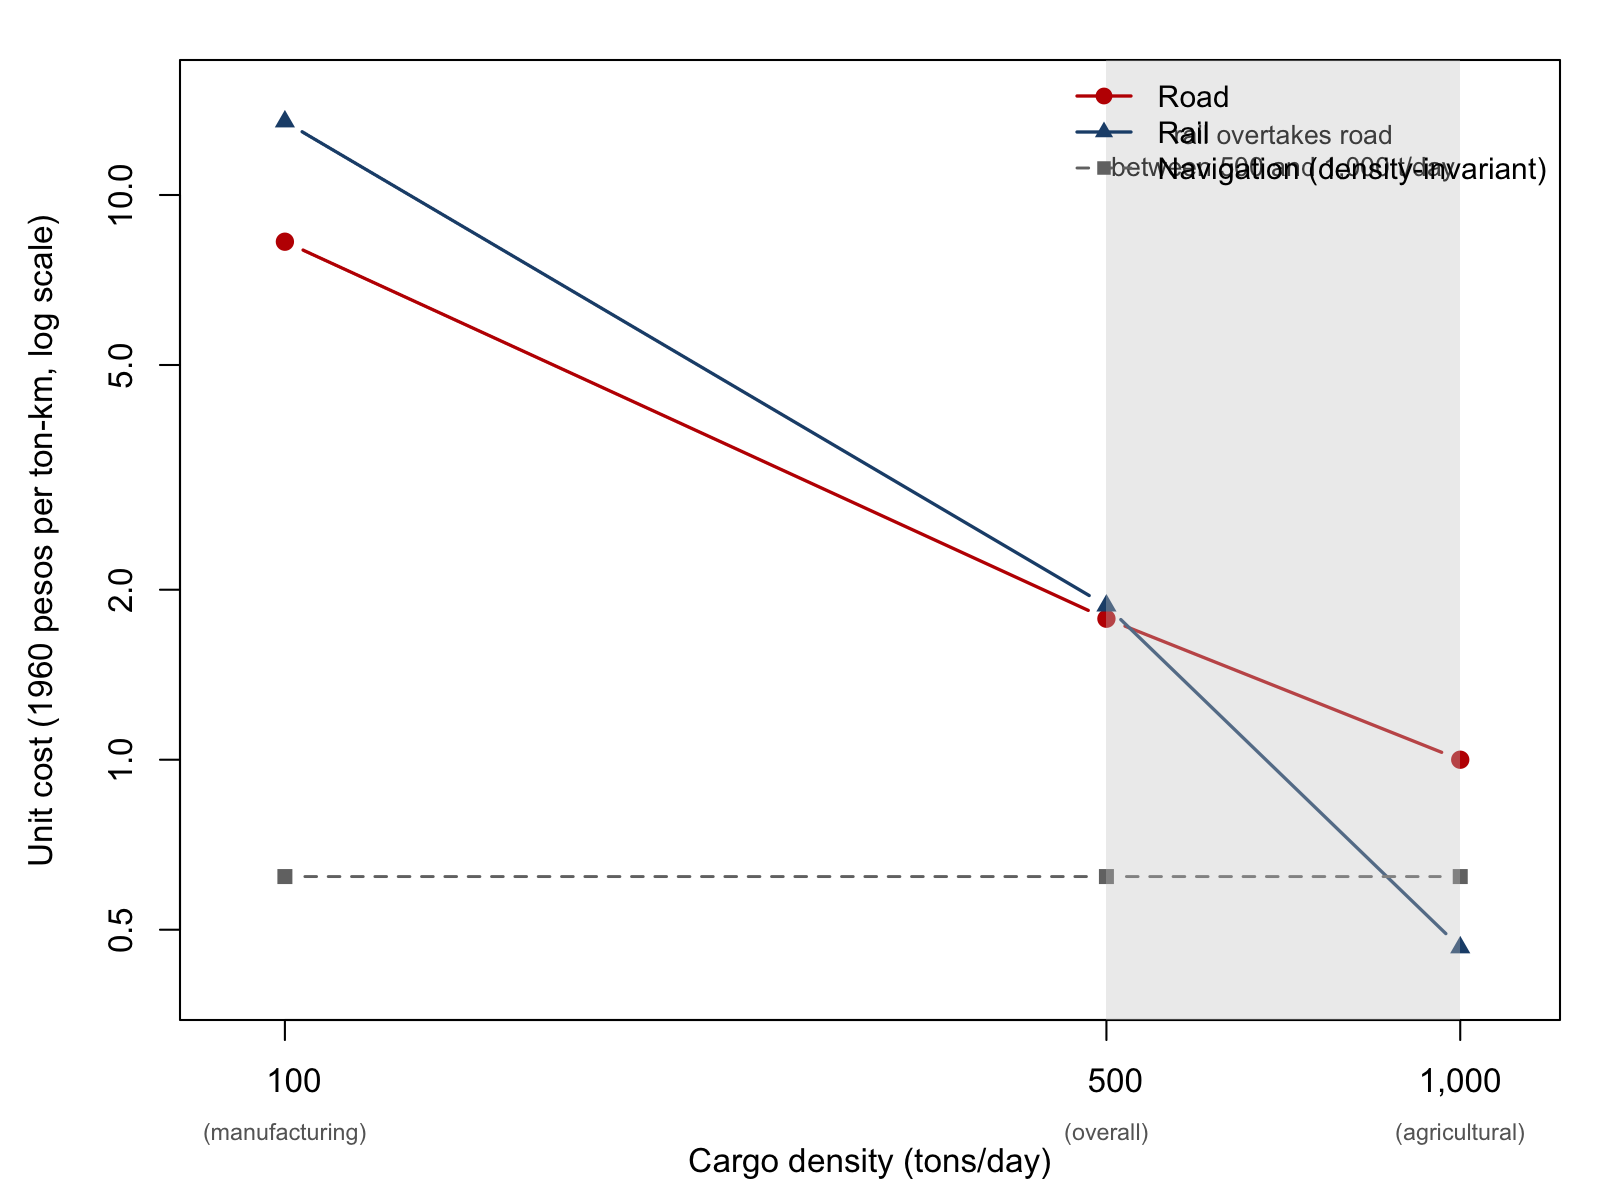
\includegraphics[width=0.8\textwidth]{figure_b1_cost_schedule.pdf}
\caption{Transport cost per ton-kilometer by mode and cargo density,
from \citet{baumgartnerpalazzo1969}.}
\label{fig:cost_schedule}
\end{figure}

\begin{figure}[htbp]
\centering
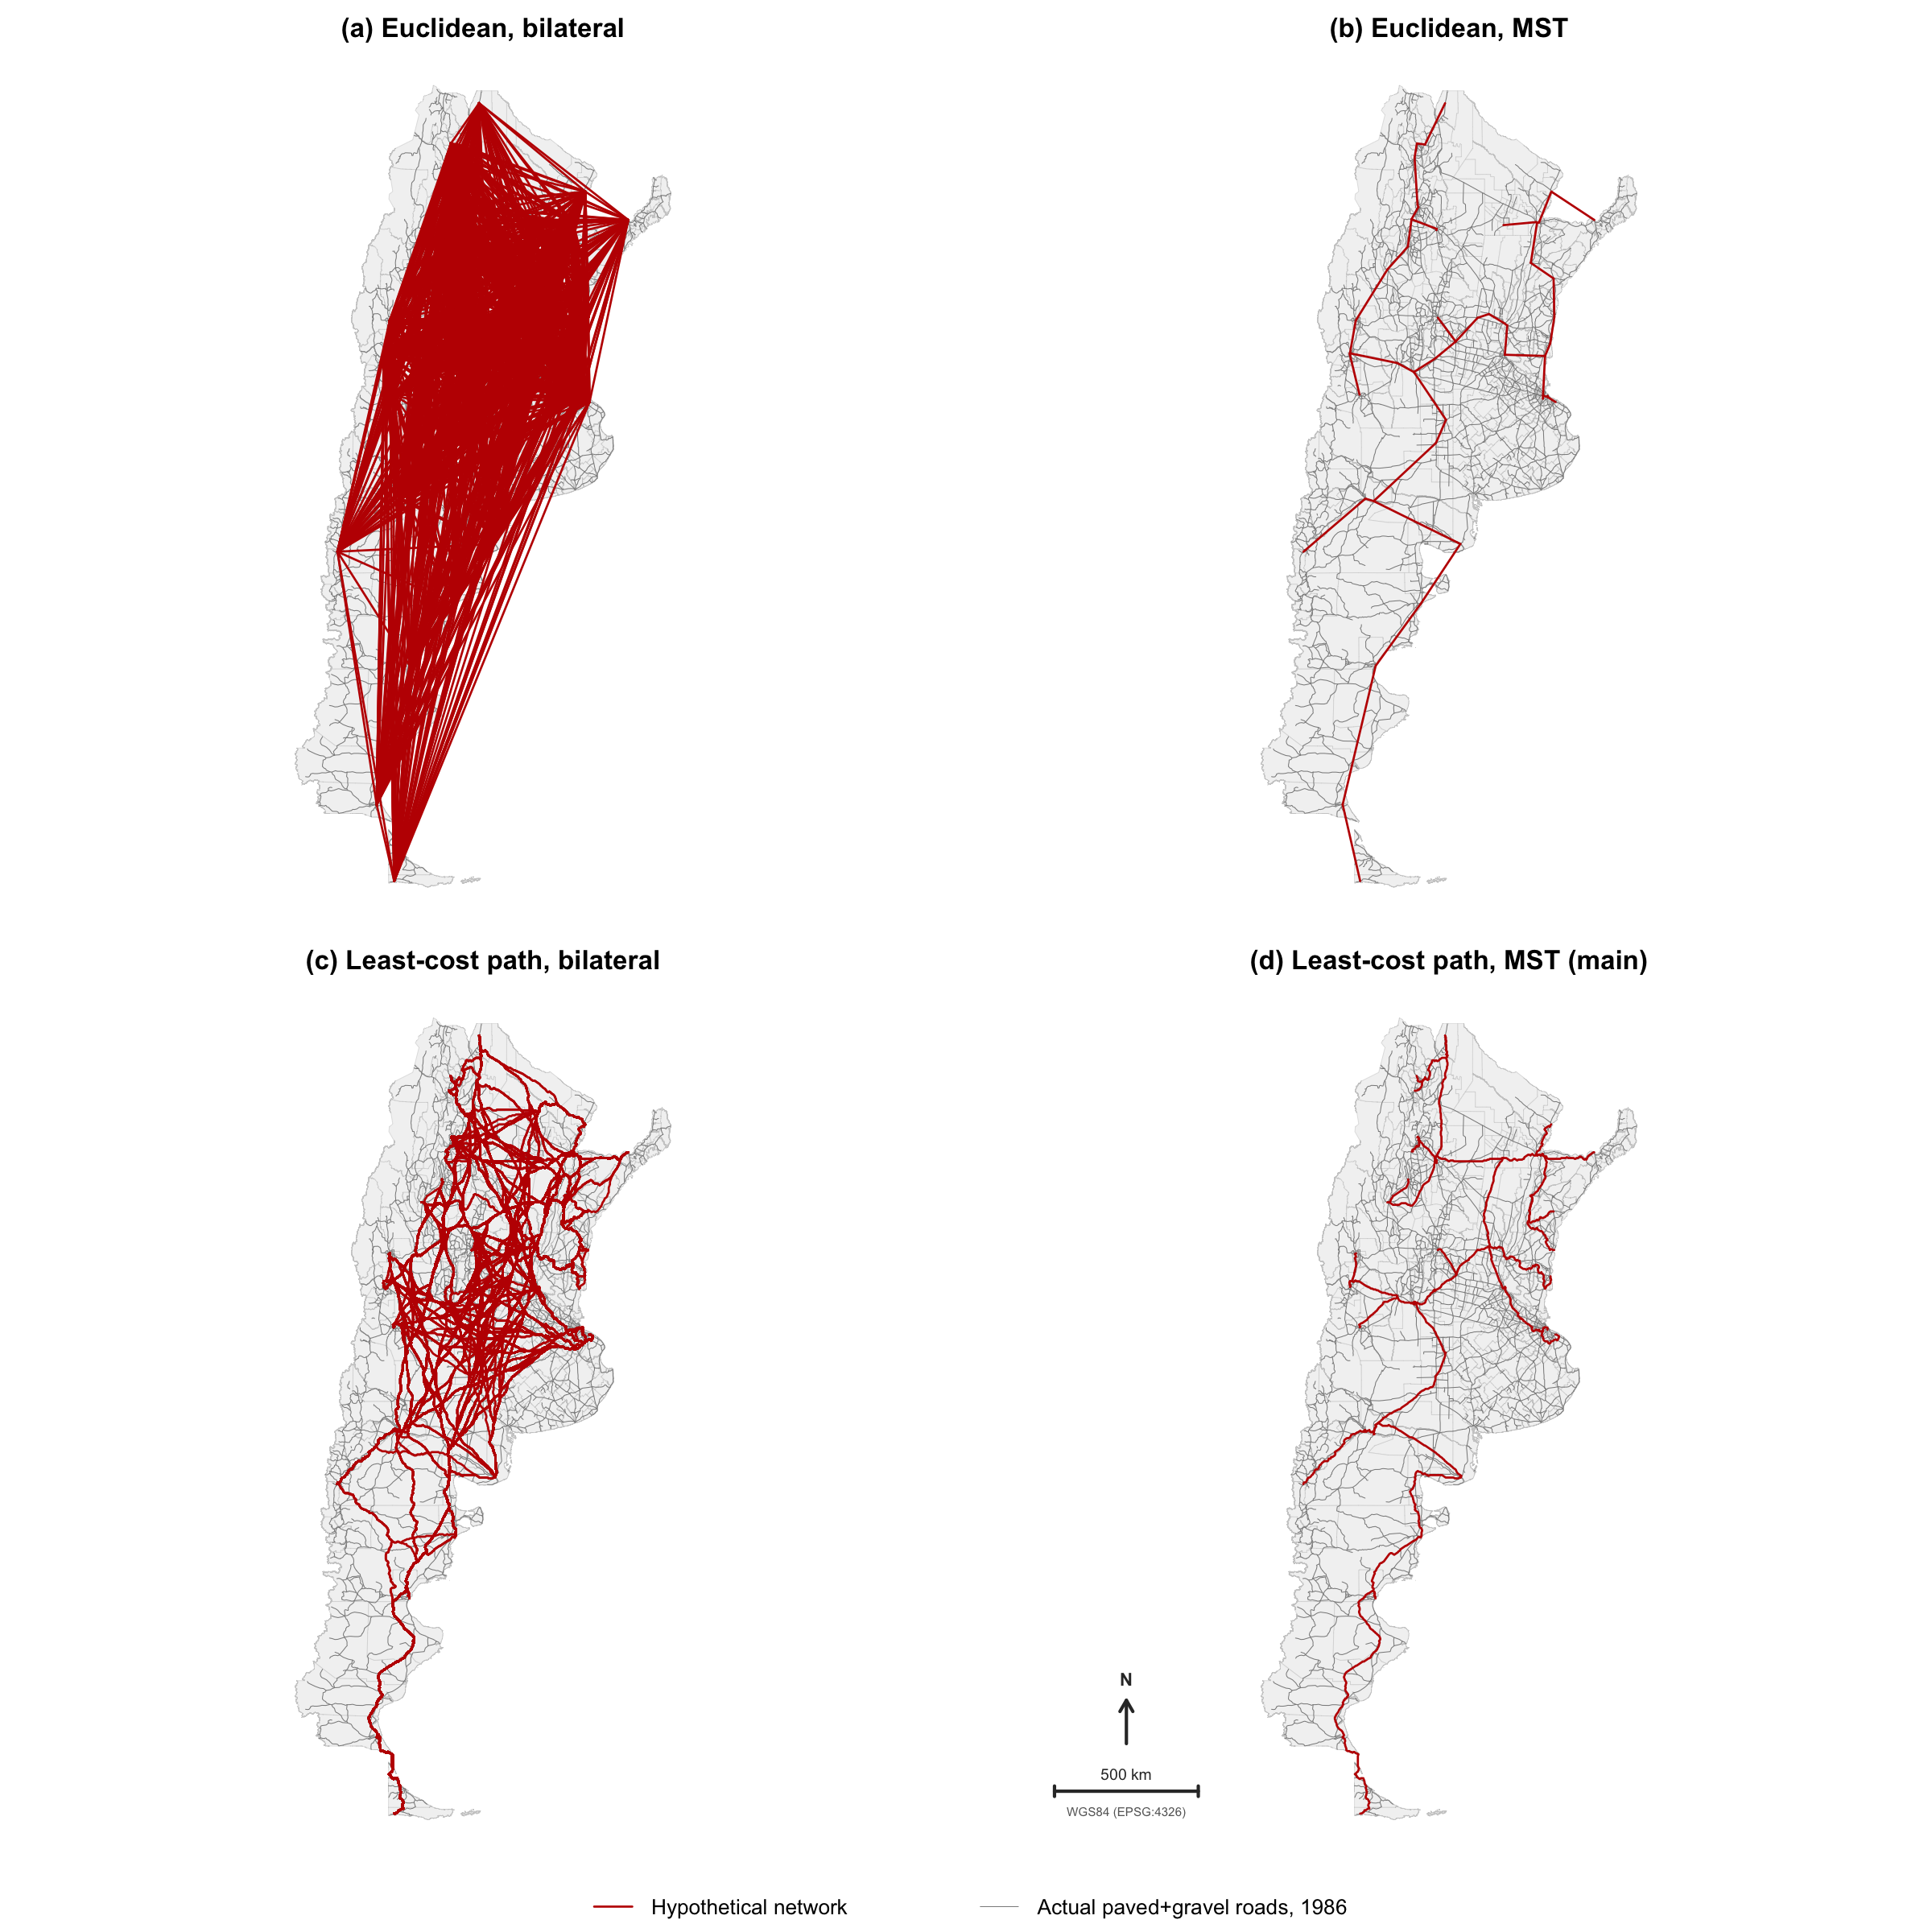
\includegraphics[width=0.85\textwidth]{figure_b2_hypothetical_networks.png}
\caption{Hypothetical road networks used by instrument 2:
least-cost-path and Euclidean variants connecting the major cities.}
\label{fig:hypo_networks}
\end{figure}

\begin{figure}[htbp]
\centering
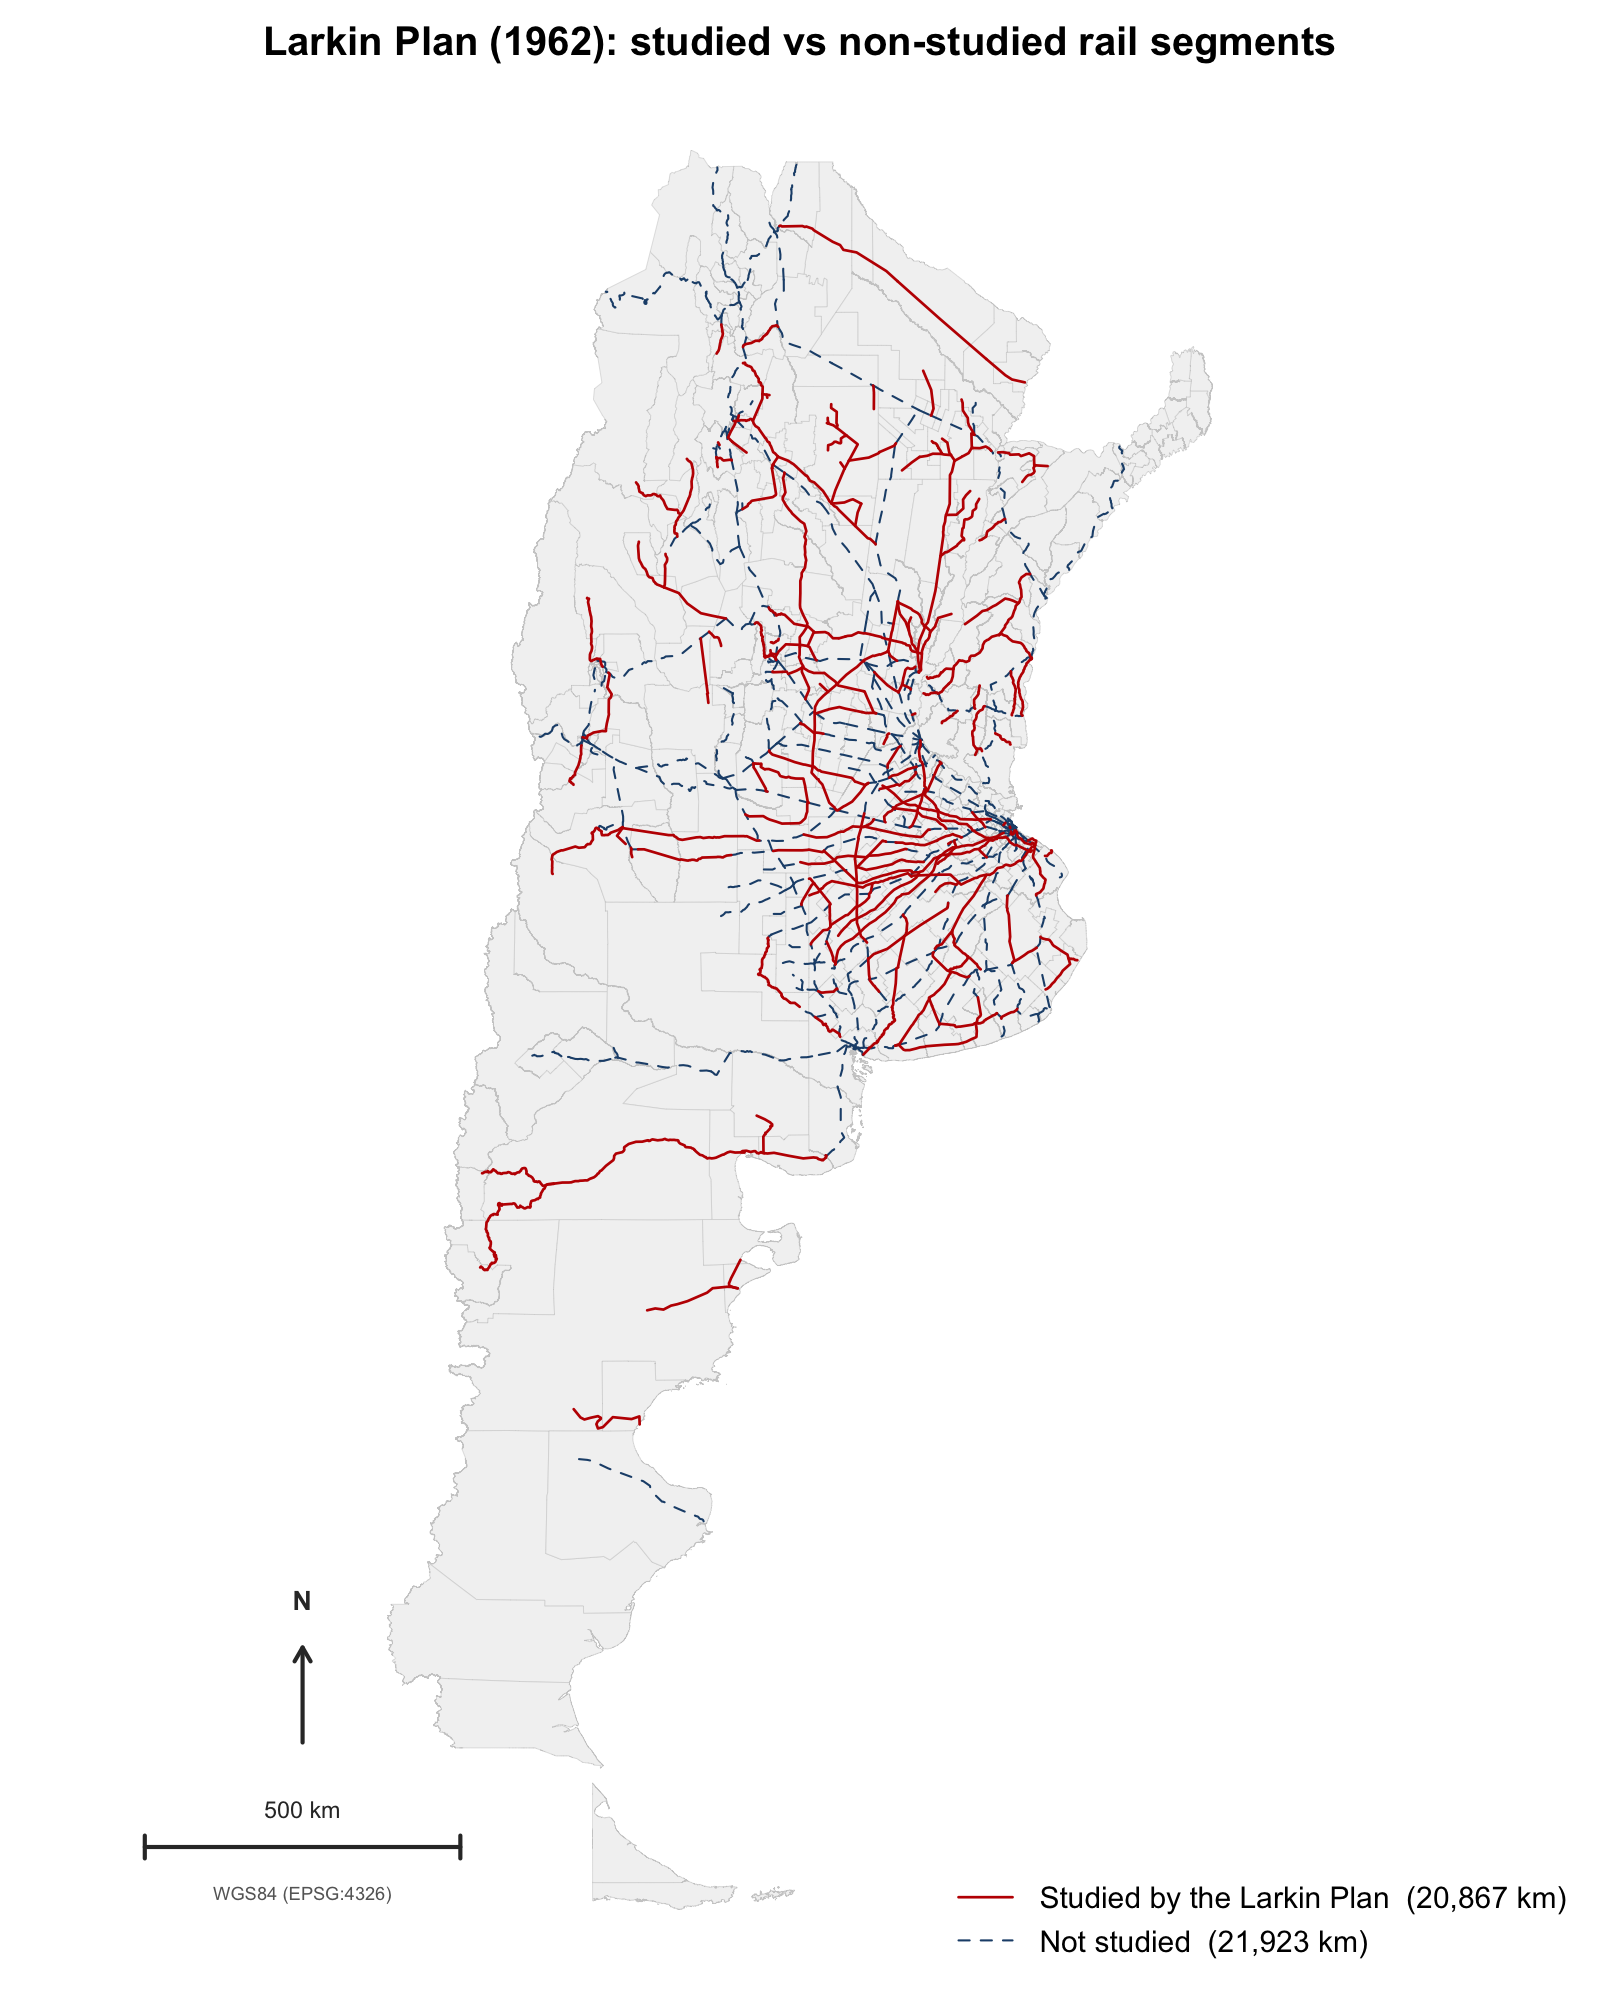
\includegraphics[width=0.85\textwidth]{figure_b3_larkin_studied.png}
\caption{Rail segments studied versus not studied by the Larkin Plan,
from the digitized plan tables.}
\label{fig:larkin_studied}
\end{figure}

\begin{figure}[htbp]
\centering
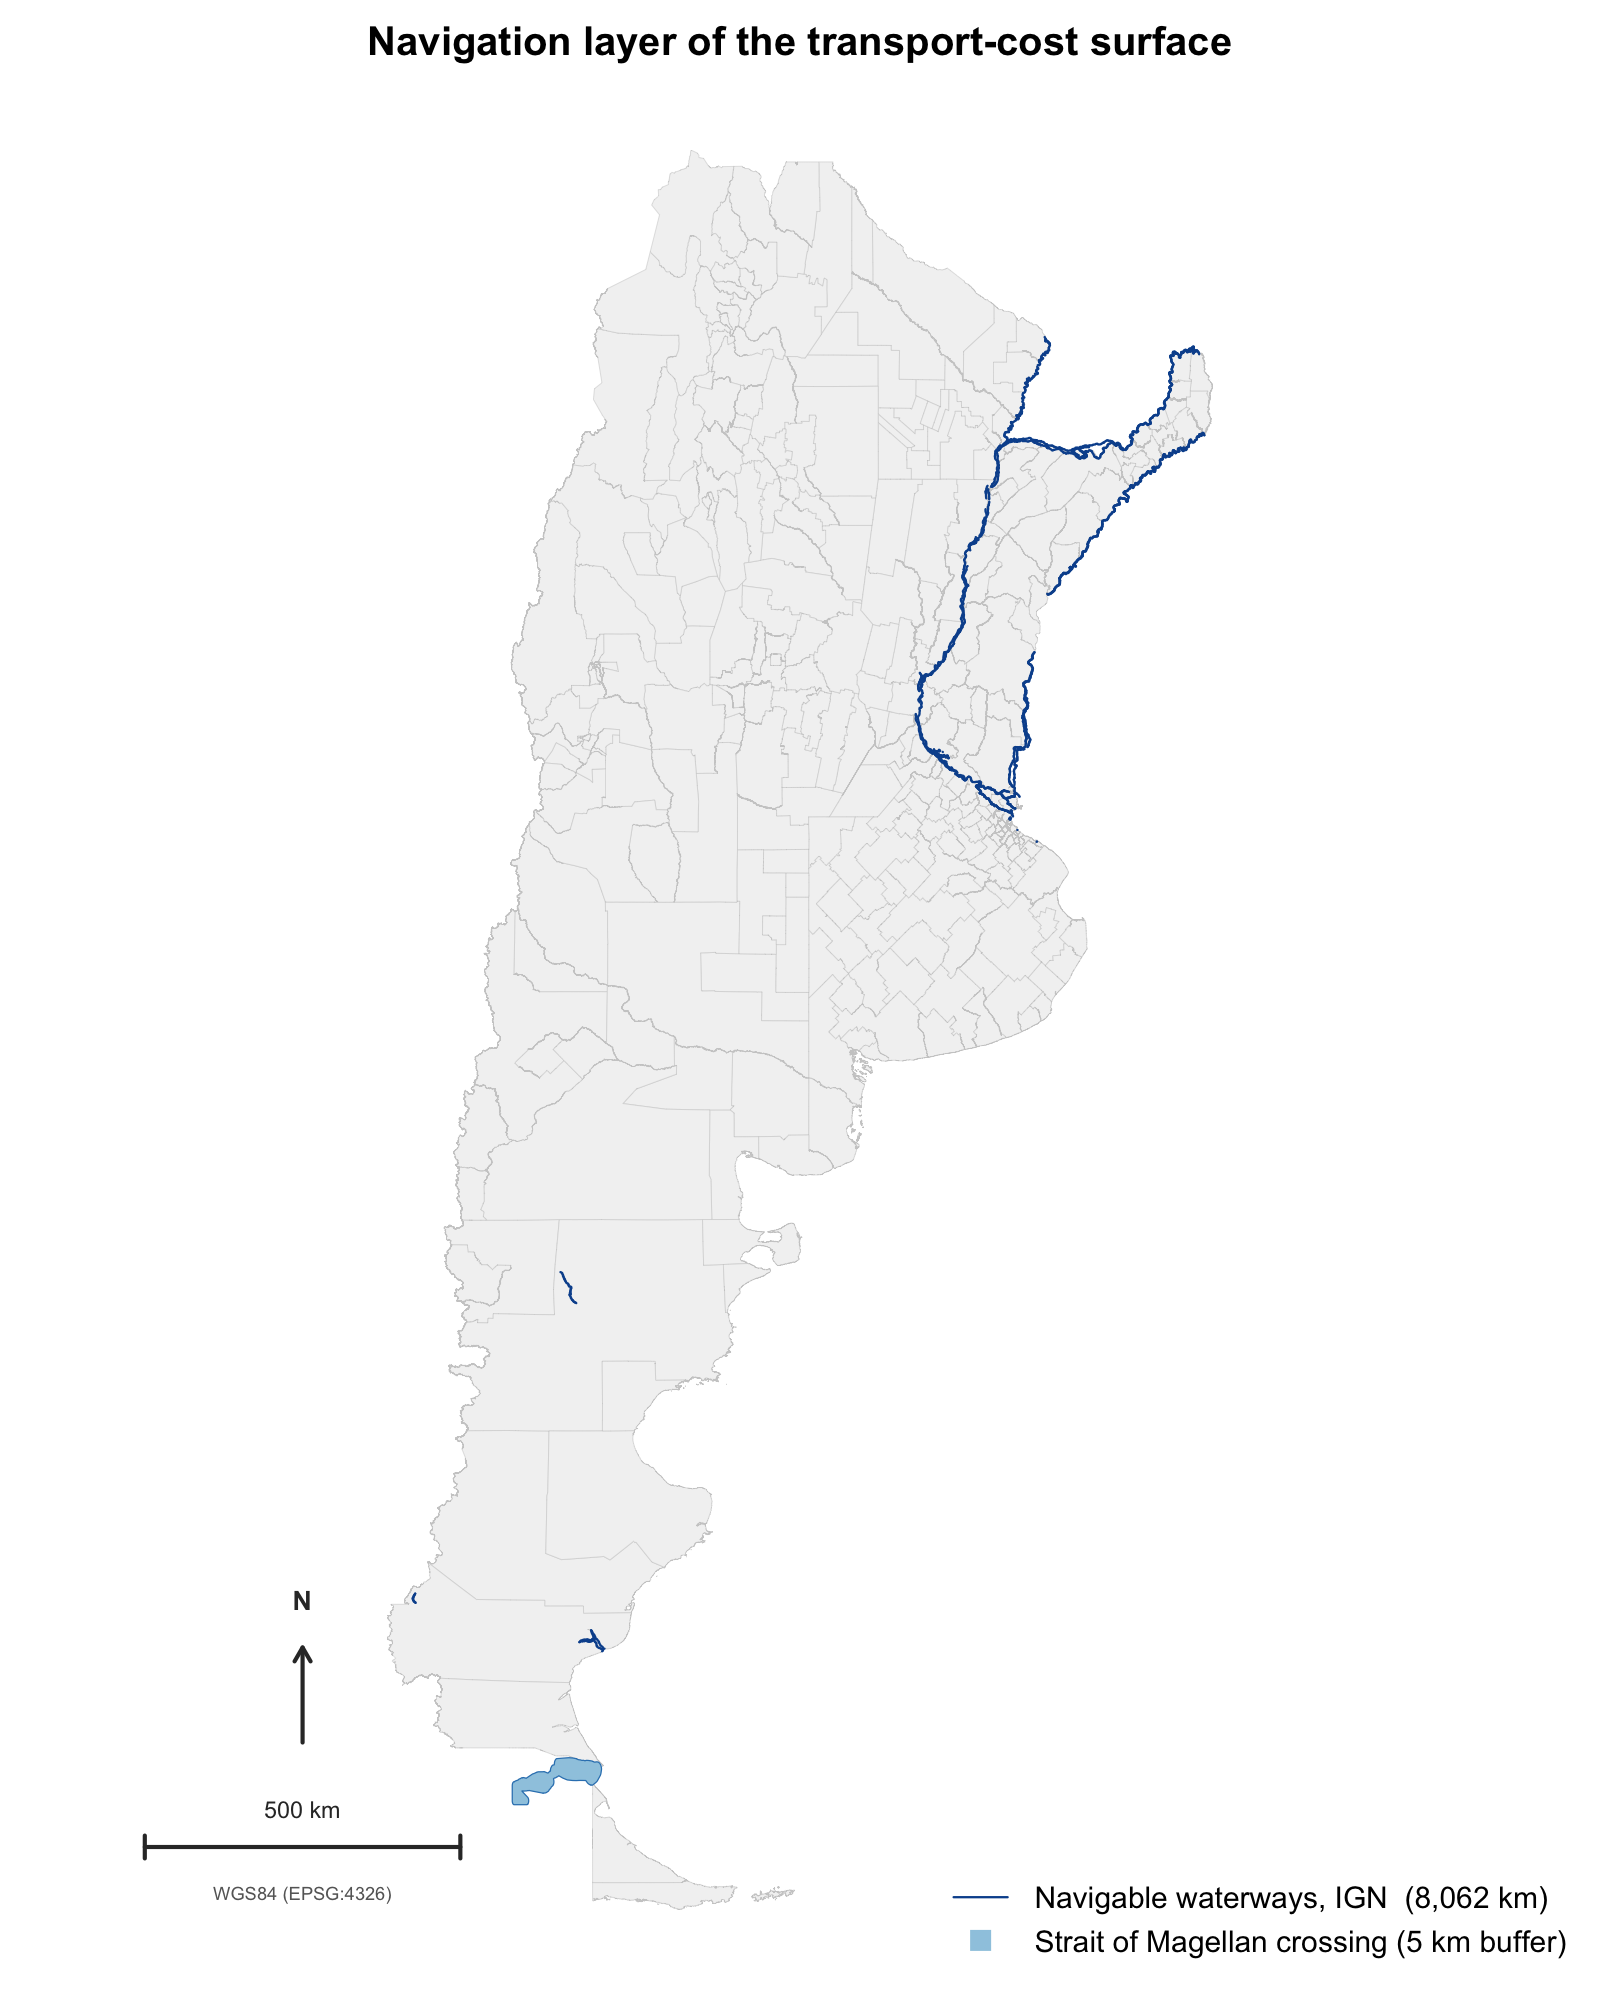
\includegraphics[width=0.85\textwidth]{figure_b4_navigation.png}
\caption{Navigation layer of the transport-cost surface: the
navigable inland waterways flagged in the IGN hydrography
\citep{ignhydro} --- the Paran\'a--Paraguay--Uruguay--R\'io de la
Plata system and a few Patagonian rivers --- and the buffered
Strait of Magellan crossing. Waterways are drawn as line geometries;
the cost surface buffers them by 1~km when rasterising. The cost
surface contains no open-ocean coastal shipping; Atlantic ports
connect through land or river legs only.}
\label{fig:navigation}
\end{figure}

\end{document}
